%Input preamble
%Style
\documentclass[12pt]{article}
\usepackage[top=1in, bottom=1in, left=1in, right=1in]{geometry}
\parindent 22pt
\usepackage{fancyhdr}

%Packages
\usepackage{adjustbox}
\usepackage{amsmath}
\usepackage{amsfonts}
\usepackage{amssymb}
\usepackage{bm}
\usepackage[table]{xcolor}
\usepackage{tabu}
\usepackage{color,soul}
\usepackage{makecell}
\usepackage{longtable}
\usepackage{multirow}
\usepackage[normalem]{ulem}
\usepackage{etoolbox}
\usepackage{graphicx}
\usepackage{tabularx}
\usepackage{ragged2e}
\usepackage{booktabs}
\usepackage{caption}
\usepackage{fixltx2e}
\usepackage[para, flushleft]{threeparttablex}
\usepackage[capposition=top,objectset=centering]{floatrow}
\usepackage{subcaption}
\usepackage{pdfpages}
\usepackage{pdflscape}
\usepackage{natbib}
\usepackage{bibunits}
\definecolor{maroon}{HTML}{990012}
\usepackage[colorlinks=true,linkcolor=maroon,citecolor=maroon,urlcolor=maroon,anchorcolor=maroon]{hyperref}
\usepackage{marvosym}
\usepackage{makeidx}
\usepackage{tikz}
\usetikzlibrary{shapes}
\usepackage{setspace}
\usepackage{enumerate}
\usepackage{rotating}
\usepackage{tocloft}
\usepackage{epstopdf}
\usepackage[titletoc]{appendix}
\usepackage{framed}
\usepackage{comment}
\usepackage{xr}
\usepackage{titlesec}
\usepackage{footnote}
\usepackage{longtable}
\newlength{\tablewidth}
\setlength{\tablewidth}{9.3in}
\setcounter{secnumdepth}{4}

\titleformat{\paragraph}
{\normalfont\normalsize\bfseries}{\theparagraph}{1em}{}
\titlespacing*{\paragraph}
{0pt}{3.25ex plus 1ex minus .2ex}{1.5ex plus .2ex}
\makeatletter
\pretocmd\start@align
{%
  \let\everycr\CT@everycr
  \CT@start
}{}{}
\apptocmd{\endalign}{\CT@end}{}{}
\makeatother
%Watermark
\usepackage[printwatermark]{xwatermark}
\usepackage{lipsum}
\definecolor{lightgray}{RGB}{220,220,220}
%\newwatermark[allpages,color=lightgray,angle=45,scale=3,xpos=0,ypos=0]{Preliminary Draft}

%Further subsection level
\usepackage{titlesec}
\setcounter{secnumdepth}{4}
\titleformat{\paragraph}
{\normalfont\normalsize\bfseries}{\theparagraph}{1em}{}
\titlespacing*{\paragraph}
{0pt}{3.25ex plus 1ex minus .2ex}{1.5ex plus .2ex}

\setcounter{secnumdepth}{5}
\titleformat{\subparagraph}
{\normalfont\normalsize\bfseries}{\thesubparagraph}{1em}{}
\titlespacing*{\subparagraph}
{0pt}{3.25ex plus 1ex minus .2ex}{1.5ex plus .2ex}

%Functions
\DeclareMathOperator{\cov}{Cov}
\DeclareMathOperator{\corr}{Corr}
\DeclareMathOperator{\var}{Var}
\DeclareMathOperator{\plim}{plim}
\DeclareMathOperator*{\argmin}{arg\,min}
\DeclareMathOperator*{\argmax}{arg\,max}

%Math Environments
\newtheorem{theorem}{Theorem}
\newtheorem{claim}{Claim}
\newtheorem{condition}{Condition}
\renewcommand\thecondition{C--\arabic{condition}}
\newtheorem{algorithm}{Algorithm}
\newtheorem{assumption}{Assumption}
\renewcommand\theassumption{A--\arabic{assumption}}
\newtheorem{remark}{Remark}
\renewcommand\theremark{R--\arabic{remark}}
\newtheorem{definition}[theorem]{Definition}
\newtheorem{hypothesis}[theorem]{Hypothesis}
\newtheorem{property}[theorem]{Property}
\newtheorem{example}[theorem]{Example}
\newtheorem{result}[theorem]{Result}
\newenvironment{proof}{\textbf{Proof:}}{$\bullet$}

%Commands
\newcommand\independent{\protect\mathpalette{\protect\independenT}{\perp}}
\def\independenT#1#2{\mathrel{\rlap{$#1#2$}\mkern2mu{#1#2}}}
\newcommand{\overbar}[1]{\mkern 1.5mu\overline{\mkern-1.5mu#1\mkern-1.5mu}\mkern 1.5mu}
\newcommand{\equald}{\ensuremath{\overset{d}{=}}}
\captionsetup[table]{skip=10pt}
%\makeindex

\setlength\parindent{20pt}
\setlength{\parskip}{0pt}

\newcolumntype{L}[1]{>{\raggedright\let\newline\\\arraybackslash\hspace{0pt}}m{#1}}
\newcolumntype{C}[1]{>{\centering\let\newline\\\arraybackslash\hspace{0pt}}m{#1}}
\newcolumntype{R}[1]{>{\raggedleft\let\newline\\\arraybackslash\hspace{0pt}}m{#1}}



%Logo
%\AddToShipoutPictureBG{%
%  \AtPageUpperLeft{\raisebox{-\height}{
\includegraphics[width=1.5cm]{uchicago.png}}}
%}

\newcolumntype{L}[1]{>{\raggedright\let\newline\\\arraybackslash\hspace{0pt}}m{#1}}
\newcolumntype{C}[1]{>{\centering\let\newline\\\arraybackslash\hspace{0pt}}m{#1}}
\newcolumntype{R}[1]{>{\raggedleft\let\newline\\\arraybackslash\hspace{0pt}}m{#1}}

\newcommand{\mr}{\multirow}
\newcommand{\mc}{\multicolumn}

%\newcommand{\comment}[1]{}

%Other parameters
\newcommand{\noutcomes}{95}
\newcommand{\noutcomesexpp}{357}
\newcommand{\noutcomesexpm}{343}
\newcommand{\noutcomesexpf}{355}
\newcommand{\treatsubsabc}{$75\%$}
\newcommand{\treatsubscarec}{$74\%$}
\newcommand{\treatsubscaref}{$63\%$}

%Counts
%Males
\newcommand{\positivem}{$78\%$}
\newcommand{\positivesm}{$29\%$}

%Females
\newcommand{\positivef}{$78\%$}
\newcommand{\positivesf}{$31\%$}

%Counts, control substitution
%Males
\newcommand{\positivecsnm}{$47\%$}
\newcommand{\positivescsnm}{$15\%$}

\newcommand{\positivecsam}{$79\%$}
\newcommand{\positivescsam}{$29\%$}

%Females
%% no alternative
\newcommand{\positivecsnf}{$84\%$}
\newcommand{\positivescsnf}{$55\%$}

%% alternative
\newcommand{\positivecsaf}{$79\%$}
\newcommand{\positivescsaf}{$33\%$}

%Pooled

%Effects
%Males

%Females
\newcommand{\empf}{$8$}
\newcommand{\yearsedf}{$1.7$}



%Pooled

%CBA
%IRR
%Males
\newcommand{\irrm}{$15\%$}
\newcommand{\irrsem}{$5\%$}

%Females
\newcommand{\irrf}{$9\%$}
\newcommand{\irrsef}{$7\%$}

%Pooled
\newcommand{\irrp}{$13\%$}
\newcommand{\irrsep}{$5\%$}

%BC
%Males
\newcommand{\bcm}{$11.24$}
\newcommand{\bcsem}{$4.60$}

%Females
\newcommand{\bcf}{$2.35$}
\newcommand{\bcsef}{$1.09$}

%Pooled
\newcommand{\bcp}{$5.63$}
\newcommand{\bcsep}{$2.15$}

%NPV streams
%Pooled
\newcommand{\parincomenpvp}{$\$119,346$}

\externaldocument{abc_comprehensivecba_appendix}
\pagenumbering{roman}

\begin{document}

\title{\Large \textbf{Analyzing the Short- and Long-term Effects of Early Childhood Education on Multiple Dimensions of Human Development}\thanks{This research was supported in part by the American Bar Foundation; the Pritzker Children's Initiative, the
Buffett Early Childhood Fund, NIH grants NICHD R37HD065072, NICHD R01HD54702, and NIA R24AG048081, an
anonymous funder, Successful Pathways from School to Work, an initiative of the University of Chicago's Committee
on Education funded by the Hymen Milgrom Supporting Organization, and the Human Capital and Economic
Opportunity Global Working Group, an initiative of the Center for the Economics of Human Development, affiliated with
the Becker Friedman Institute for Research in Economics, and funded by the Institute for New Economic Thinking. The
views expressed in this paper are solely those of the authors and do not necessarily represent those of the funders or
the official views of the National Institutes of Health. Collaboration with Yu Kyung Koh, Sylvi Kuperman, Stefano Mosso, Rodrigo Pinto, and Anna Ziff on related work has strengthened the analysis in this paper. For helpful comments, we thank St\'{e}phane Bonhomme, Fl\'{a}vio Cunha, Steven Durlauf, Azeem Shaikh, Matthew Tauzer, and Ed Vytlacil. For information on the implementation of the Carolina Abecedarian Project and assistance in data acquisition, we thank Peg Burchinal, Carrie Bynum, Frances Campbell, and Elizabeth Gunn. For information on childcare in North Carolina, we thank Richard Clifford and Sue Russell.}}

\author{
Jorge Luis Garc\'{i}a\\
The University of Chicago \and
James J. Heckman \\
American Bar Foundation \\
The University of Chicago \and
Andr\'{e}s Hojman\\
The University of Chicago \and
Duncan Ermini Leaf \\ 
University of Southern California \and
Mar\'{i}a Jos\'{e} Prados \\
University of Southern California \and
Joshua Shea \\
The University of Chicago \and 
Jake C. Torcasso\\
The University of Chicago}
\date{First Draft: January 5, 2016\\ This Draft: \today}
\maketitle
\thispagestyle{empty}

\doublespacing
\begin{abstract}
\noindent This paper uses data from two high-quality randomized controlled trials and multiple non-experimental sources to provide a life-cycle cost-benefit analysis of early childhood education programs, as well as an understanding of its components. We define and estimate parameters that have a link with different policy-evaluation questions. We explore the outcome categories that are most important when accounting for the programs' costs and benefits and formalize an alternative to the standard solution to multiple hypothesis testing \citep{Lehman_Romano_2005_AnnStat,Romano_Shaikh_2006_AnnStat}. We conclude that early childhood education programs are socially efficient by documenting a benefit-to-cost ratio of \bcp\  (s.e. \bcsep) and an internal rate of return of \irrp\  (s.e. \irrsep). We perform sensitivity analysis and find that these estimates are robust to various perturbations of the parameters and assumptions in the cost-benefit analysis.
\end{abstract} 

\singlespacing
%\pagebreak
\tableofcontents
\listoffigures
\listoftables
%\pagebreak
\doublespacing

\pagebreak
\setcounter{page}{0}
\pagenumbering{arabic}

\section{Introduction}

\noindent There is a growing interest in early childhood education as a means for promoting social mobility.\footnote{\citet{Bajaj_Labaton_2009_ObamaRiskAssets,White_House_2014_Econ_of_EC_Investments,White_House_2014_Fact_Sheet_Press}.} Overall state-spending on such programs increased by 12 percent in 2015. The proposed federal budget for 2017 includes a \$300 million increase in spending on early childhood education.\footnote{\citet{US-Gov_2016_Budget,Parker-etal_2016_50-State-Review,Smith_2016_Early-Learning-Budget}.}\\

\noindent Despite the growing emphasis on early childhood education in public policy, comprehensive and methodologically rigorous evidence on its economic benefits is still scarce. Many recent studies: (i) focus on a limited set of outcomes that fail to capture a comprehensive array of program effects;\footnote{An extreme example is the evaluation of preschool programs using an age-eligibility cutoff. A battery of studies compare children who were just eligible and just ineligible for preschool. They therefore only assess the gains of an additional, earlier year of preschool. This does not represent a comprehensive evaluation approach; it evaluates a specific set of children for a very narrow set of tests and within a time horizon of a single year of treatment. Examples of these studies include: \citet{Gormley_Gayer_2005_JHR,Gormley_Gayer_etal_2005_DP,Weiland_2013_CD_Impacts-of-Pre-K}.} (ii) are based on data from follow-ups that are short-term in nature; (iii) do not correct for program attrition or for non-compliance to assigned treatment, threatening the policy-relevance of their estimates;\footnote{Consider the evaluation of Head Start through its randomized controlled trial, the Head Start Impact Study \citep{Puma_Bell_etal_2010_HeadStartImpact}. Comparing subjects in the treatment and the control groups usually yields relatively low gains. This attenuation happens because a substantial proportion of subjects randomized out of the program were enrolled into preschool alternatives, some of them to other Head Start centers. Thus, a raw comparison between the treatment- and the control-group subjects does not inform on either the efficiency or the effectiveness of Head Start \emph{per se}. Studies providing a methodology to account for substitution find that Head Start has substantial effects, although they focus on a single, short-term outcome \citep{Kline-Walters_2015_NBER-Evaluating,Feller_Grindal_etal_2016_ComparedtoWhat}.} or (iv) are based on randomized controlled trials with flawed designs.\footnote{An evaluation of the Tennessee Voluntary Prekindergarten is an example \citep{Lipsey_et_al_2013_Tennessee_Kindergrtn_PRI,Lipsey_et_al_2015_Randomized_Control_Trial_PRI}. The researchers designed a randomized controlled trial to evaluate the program. Unfortunately, they asked permission to assess the children after the randomization protocol. Thus, their main evaluation is based on information for children whose parents agreed for them to be evaluated \textit{post} randomization, inducing a potential imbalance between the children randomized into and out of the program. The evaluation does not account for that. Further, results for this evaluation represent a narrow set of short-term outcomes.}\\ 

\noindent  Current justification for the long-term effectiveness and the efficiency of early childhood education in the U.S. is largely based on evidence from the Perry Preschool Program (referred to simply as Perry). Analyses of Perry suggest that early childhood education has significant positive effects on multiple short- and long-term socio-economic outcomes, even when accounting for compromised randomization, small-sample-size inference, and multiple hypothesis testing \citep{Heckman_Moon_etal_2010_QE}. The analyses also show that early childhood education could have an annual internal rate of return that ranges from 7 to 10 percent.\footnote{That is, if one dollar were to be invested at age 4, and then reinvested annually and compounded over a lifetime, the return would accrue to 60 to 300 dollars by age 65. This accounts for both the program's cost and the social burden a government would cause by raising taxes to pay for it \citep{Heckman_Moon_etal_2010_RateofReturn}.}\\

\noindent One of the criticisms of the empirical evidence favoring the economic case for early childhood education is the lack of an ampler evidence base. In response, we analyze both short- and long-term effects of early childhood education on multiple dimensions of human development using data from two randomized controlled trials, the Carolina Abecedarian Project (ABC) and the Carolina Approach to Responsive Education (CARE)---we complement this data with several non-experimental, nationally representative sources.\\

\noindent ABC and CARE were programs implemented in the 1970s and early 1980s. We observe short- and long-term outcomes for the subjects. The programs were separated into two phases. In the first phase, both programs randomly assigned subjects to high-quality center-based childcare from ages 0 to 5. In addition, the subjects who were assigned to center-based childcare in CARE also received home visits that aimed to foster the relationship between the subjects and their parents. Furthermore, CARE incorporated a second treatment group that received home visits without center-based childcare from ages 0 to 5. The second phase of treatment, from ages 5 to 8, consisted of home visits that aimed to continue promoting childhood development. In ABC, the second-phase treatment was randomly assigned independently of the first-phase randomization. In CARE, the second-phase was not randomized; subjects initially randomized to either of the treatment groups maintained their assignment.\footnote{Our main evidence is based on the first-phase component that the two programs share: high-quality center-based childcare. We offer some results on first-phase home visits and the second-phase treatment as complementary.}\\

\noindent The experimental data from ABC and CARE include measures of cognitive and socio-emotional skills, educational and labor market outcomes, administrative criminal records, and a full medical examination when subjects reached their mid-30s. Data from administrative criminal records and from the full medical panel are novel to the literature evaluating early childhood education programs. The non-experimental, nationally representative data include sources to forecast life-cycle gains in public-transfer and labor income, health, and crime. Examples of these sources include: the Medical Expenditure Panel Survey (MEPS), the Medicare Current Beneficiary Survey (MCBS), and the Uniform Crime Reporting Statistics (UCRS).\\

\noindent Our ultimate goal is to provide a cost-benefit analysis of early childhood education programs.\footnote{We only perform these calculations for ABC due to data limitations---the documentation of the costs for  CARE is minimal.} To construct this, we proceed in three steps. In the first step, we begin by defining the treatment-effect parameters we estimate and state how they link to different policy questions. Our methodology accounts for different forms of attrition and non-compliance. Specifically, it considers that the parents of roughly 70\% of the children randomized out of center-based childcare enrolled their children in relatively high-quality preschool alternatives. We refer to this phenomenon as control substitution.\footnote{Control  substitution was not an issue in Perry. Informal conversations with Perry's staff indicate that there were no alternative preschools in the area in which subjects were treated during that time---Ypsilanti, Michigan during the 1960s. This issue is more pressing when evaluating recent programs. Examples include both ABC and Head Start---see \citep{Puma_Bell_etal_2010_HeadStartImpact} for a documentation of treatment substitution in the Head Start Impact Study.}\\

\noindent In the second and intermediate step, we provide treatment-effect estimates for a wide variety of outcomes. In doing so, a challenge arises: we test multiple hypotheses. We account for this in a standard way \citep{Lehman_Romano_2005_AnnStat,Romano_Shaikh_2006_AnnStat} while noting that it is often the case that arbitrary blocks need to be formed in order to adjust the inference using the step-down procedure. We propose and formalize an alternative: count the positive (and significant) treatment effects across the outcomes we consider. This crude summary highlights which outcome categories have the most effects, and therefore are relevant to the cost-benefit analysis, which then weighs the relative importance of each outcome.\\ 

\noindent Finally, to conduct the cost-benefit analysis, we combine the experimental and non-experimental sources of data to forecast and monetize parental income, transfer income, labor income, education, health, and crime outcomes over the life-cycle to provide estimates of the benefit-to-cost ratio and the internal rate of return of early childhood education. Because these statistics summarize the effectiveness of a program accounting for all its components in a single statistic (and a single inference test), they provide a comprehensive solution for the challenge of performing multiple hypothesis testing.\\

\noindent ABC's and CARE's center-based childcare from ages 0 to 5 as implemented, had substantial treatment effects on a comprehensive set of measures of human development from childhood through adulthood. For females, \positivef\ of the outcomes we study have a \textit{positive} average treatment effect; \positivesf\ of the outcomes we study have a \textit{positive and significant} average treatment effect, at the 10\% level. For males, the analogous figures are \positivem\ and \positivesm.\footnote{These results account for program attrition.} The effects strengthen when accounting for control substitution by the families of the subjects who were randomized out of the main treatment  the programs offered.\\

\noindent This paper extends the work of \citet{Campbell_Conti_etal_2014_EarlyChildhoodInvestments}, who analyze the effectiveness of ABC at improving long-term health outcomes. We extend the analysis by (i) assessing multiple measures of human development; (ii) accounting for control substitution; and (iii) providing an alternative to test multiple hypotheses.\footnote{\cite{Campbell_Pungello_etal_2012_DP} also precede our work. The authors estimate treatment effects on adulthood outcomes in ABC. Unlike our approach, the authors do not assess outcomes such as health status, criminal behavior, and socio-emotional skills.} Furthermore, we complement the analysis by studying ABC together with CARE.\\ 

\noindent The cost-benefit analysis of ABC provides composite measures of the program's efficiency that weigh these treatment effects according to their cost to society. The pooled benefit-to-cost ratio, \bcp\ (s.e. \bcsep), and internal rate of return \irrp\ (s.e. \irrsep), indicate that ABC is an efficient program when considering the life-cycle trajectories of the subjects. \\

\noindent Two previous related pieces of work provide a cost-benefit analysis of ABC \citep{Masse_Barnett_2002_BOOKBenefitCostAnalysis,Barnett_Masse_2007_EER}. Their analysis is limited to outcomes up to age 21, before any of the labor income, crime, and health benefits of the program arise according to our findings. It does not provide standard errors or an analysis of the estimates' sensitivity to different modeling assumptions. \citet{Kline-Walters_2015_NBER-Evaluating} provide a back-of-the-envelope cost-benefit analysis of Head Start using the Head Start Impact Study. They do not analyze the life-cycle benefits and costs of early childhood education.\footnote{We present our own back-of-the-envelope cost-benefit analysis in Appendix~\ref{appendix:back}. It is in the same spirit to that of \citet{
Kline-Walters_2015_NBER-Evaluating}. It considers only the gains on labor income implied by the gain in kindergarten IQ proposed by \citet{
Chetty_Friedman_etal_2011_QJoE}. We find that the benefit-to-cost ratio is $0.4$. This reinforces the idea that a comprehensive evaluation of the costs and benefits needs to consider multiple dimensions of human capital, and not only the labor income gains implied by short-term IQ.} \\ 

\noindent The paper proceeds as follows. Section~\ref{section:background}  provides an overview of each program. It includes a description of the eligibility criteria and the populations served, a characterization of the randomization protocol and control substitution, a comprehensive summary of the treatment, and a description of the data sources. Section~\ref{section:methodology} formalizes our methodology by discussing how we correct for compromised randomization and control substitution, how we test for treatment effects across multiple outcomes, and how we forecast outcomes across the life cycle. Section~\ref{section:results} presents our main results and Section~\ref{section:conclusion} offers some final comments. An extensive appendix presents a thorough description of the program and its costs, the data, and details on how we monetize the life-cycle outcomes. It also discusses various alternative methodologies to evaluate the programs accounting for control substitution, and documents the results we present to a further extent.

\section[Background and Data Sources]{Background and Data Sources\footnote{This section of the paper is based on joint work with Sylvi Kuperman. We expand it  in Appendix~\ref{appendix:background} and Appendix~\ref{app:programcosts}.}} \label{section:background}

\subsection{Overview}

\noindent The Carolina Abecedarian Project (ABC) and the Carolina Approach to Responsive Education (CARE) programs were designed and implemented by researchers at the Frank Porter Graham Center (FPGC) of the University of North Carolina in Chapel Hill. The programs targeted disadvantaged children from the semi-rural communities in the surrounding area. 

\noindent ABC recruited four cohorts of children born between 1972 and 1977. CARE recruited two cohorts of children, one born in 1978 and one in 1979. The recruitment process for each study was identical. Potential families were referred to researchers by local social service agencies and hospitals at the beginning of the mother's last trimester of pregnancy. Eligibility was determined by a score of 11 or above on a High-risk Index (HRI).\footnote{Examples of variables in the HRI are maternal education and father's stability at work. See Appendix~\ref{appendix:background} for details on the construction of the HRI.} \\

\noindent To better characterize the socio-economic status of the families participating in ABC and CARE, we construct two comparison groups using the Panel Study of Income Dynamics (PSID), a nationally representative cohort of children born in the same years as the ABC and CARE subjects (1972-1979), and a similar cohort restricted to black children. We show a comparison in Figure~\ref{figure:baselineabccare}. Compared to both nationally representative groups, ABC subjects were were born to younger, less educated mothers, most of whom were raising their children without the support of a father. The CARE subjects were similarly disadvantaged compared to nationally representative groups with respect to these basic household demographic characteristics.\\

\begin{figure}[H]
\caption{Family Environment Baseline Characteristics, ABC and CARE}  \label{figure:baselineabccare}
    \centering
\begin{subfigure}{.5\textwidth}
  \centering
  \subcaption{Average Maternal Age}
  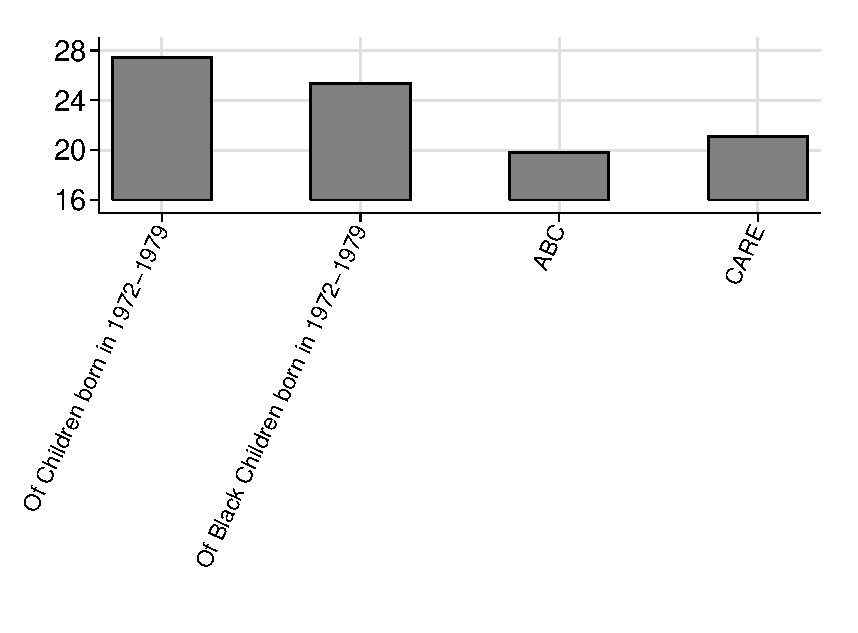
\includegraphics[height=2.3in]{output/abccarepsid_m_age0pool.eps}
\end{subfigure}%
\begin{subfigure}{.5\textwidth}
  \centering
  \subcaption{Average Maternal Years of Education} 
  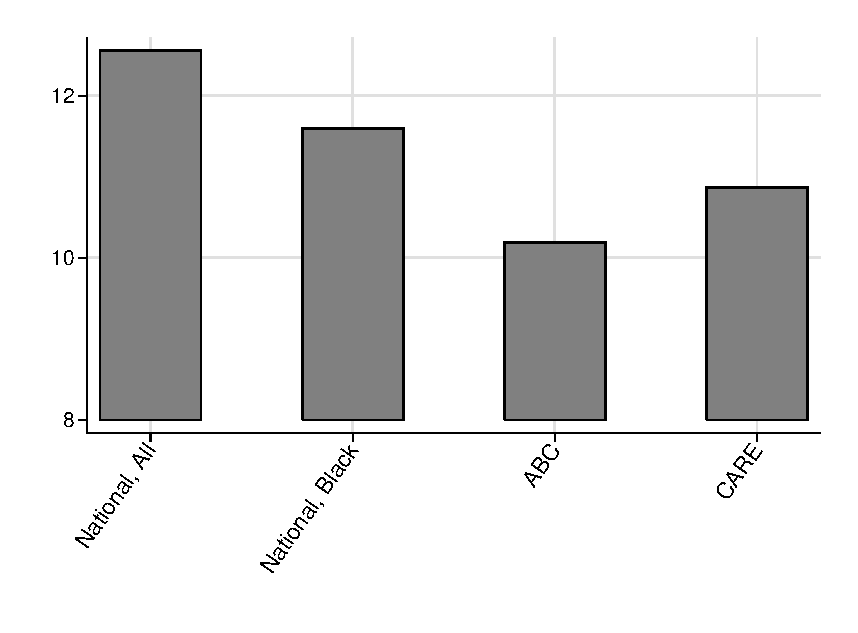
\includegraphics[height=2.3in]{output/abccarepsid_m_edu0pool.eps}
\end{subfigure}

\begin{subfigure}{.5\textwidth}
  \centering
  \subcaption{Proportion of Households with Father at Home}
  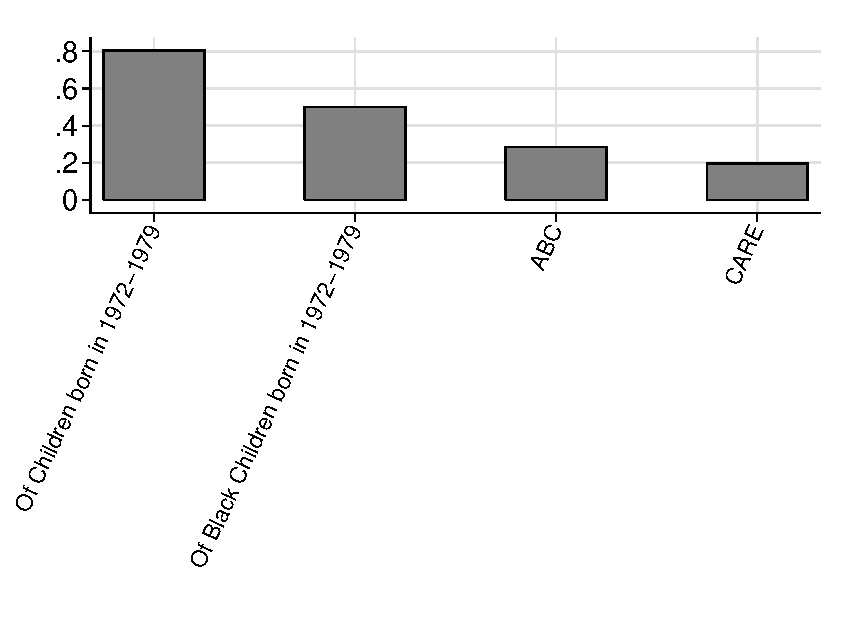
\includegraphics[height=2.3in]{output/abccarepsid_f_home0pool.eps}
\end{subfigure}%
\floatfoot{
\footnotesize
\noindent  Note: These panels plot mother's age, mother's education, and an indicator of the father's presence at home. In each panel, the first bar shows the national-level for a cohort born in the same years as the ABC and CARE subjects (1972-1979), obtained from the Panel Study of Income Dynamics (PSID). The second bar uses this same information restricted to black individuals. The third and fourth bars plot the same variables for ABC and CARE, pooling the treatment and control groups.
}
\end{figure}

\noindent The design and implementation of both programs were similar. Both studies had a small sample size. ABC recruited 122 subjects over four cohorts, while CARE recruited 67 subjects over two cohorts. ABC had two phases, the first of which lasted from birth until age 5. In this phase, children were randomly assigned to either treatment or control groups. The treatment group received: (i) center-based childcare; (ii) breakfast, lunch, an afternoon snack, iron-fortified formula for the first 15 months of life, and diapers until age 3; and (iii) medical care from licensed nurses who were supervised by a pediatrician, frequent health check-ups, and hospital referrals when serious medical treatment was needed. In contrast, the control group only received iron-fortified formula for the first 15 months and diapers until age 3. In the second phase of treatment, at the age of 5, the 95 subjects still in the study were randomly assigned again to treatment or control groups, independently of their status in the prior randomization. This second-phase treatment consisted of home visits targeting both children and parents and lasted until age 8.\\ 

\noindent  CARE also had two treatment phases, though subjects were randomized only once. While the two programs had essentially identical second phases, the first phase of CARE differed from the first phase of ABC by including a family education component. This component was designed to study the effects of improving the home environment on child development.\footnote{\citet{Wasik_Ramey_etal_1990_CD}.} The first treatment phase of CARE lasted from birth until age 5. Children were randomly assigned to one of three experimental groups: control (23 children), family education (27 children), and both family education and center-based childcare (17 children). As in ABC, the control group received iron-fortified formula from birth to 15 months and diapers to age 3. The family education group received home visits that aimed to help parents solve common problems related to childrearing. Both treatment groups received the second phase of treatment from ages 5 to 8. The ABC and CARE programs shared many objectives and program characteristics, as summarized in Table~\ref{tab:programcomparison}.

\begin{table}[H]
\begin{center}
\begin{threeparttable}
\caption{ABC and CARE, Programs Comparison} \label{tab:programcomparison}
\scriptsize
\scalebox{.9}{\begin{tabular}{L{4cm} L{7cm} L{5cm}}
\hline \hline
& \multicolumn{1}{c}{ABC}& \multicolumn{1}{c}{CARE}\\
\hline 
Program Overview &&\\
\hspace{.5cm} Years Implemented &1972--1982&1978--1985\\
\hspace{.5cm} Age of Entry/Exit & birth to 5 years old &\checkmark\\
\hspace{.5cm} Initial Sample &122&64\\
\hspace{.5cm} \# of Cohorts &4&2\\
\midrule
Eligibility & socio-economic disadvantage according to a multi-factor index (see Section \ref{section:eligibility})&\checkmark\\
 \midrule
Control &&\\
\hspace{.5cm} N &54&23\\
\hspace{.5cm} Compensation & Diapers from birth to age 3, unlimited formula from birth to 15 months & \checkmark \\
\hspace{.5cm} Treatment Substitution & 70\% & $\sim$ 70\%\\
\midrule
Treatment & Center-based childcare & Center-based childcare and family education\\
\hspace{.5cm} \textbf{Center-base} &&\\
\hspace{.5cm} \textbf{Childcare} &&\\
\hspace{.5cm} N &57&17\\
\hspace{.5cm} Intensity &6.5--9.75 hours a day for 50 weeks per year&\checkmark\\
\hspace{.5cm} Components & Instruction, medical care, nutrition, social services &\checkmark\\
\hspace{.5cm} Staff-to-child Ratio &1:3 during ages 0--1 &\checkmark\\
&1:4--5 during age 1--4 &\checkmark\\&1:5--6 during ages 4--5 &\checkmark\\
\hspace{.5cm} Staff Qualifications &Mixed diplomas; experienced&\checkmark\\
\hspace{.5cm} \textbf{Family Education} & Not part of the program &24\\
\hspace{.5cm} Intensity && One hour-long home visits. 2--3 per month during ages 0--3. 1--2 per month during ages 4--5\\
\hspace{.5cm} Curriculum & & Social and mental stimulation; parent-child interaction\\
\hspace{.5cm} Staff-to-child Ratio &&1:1\\
\hspace{.5cm} Staff Qualifications &&Home visitor training\\
\midrule
 School-age Treatment \\
 \hspace{.5cm} N&46&39\\
\hspace{.5cm} Intensity &Every other week& \checkmark\\
\hspace{.5cm} Components &Parent-teacher meetings& \checkmark\\
\hspace{.5cm} Curriculum & Reading and math &\checkmark\\
\hspace{.5cm} Staff-to-child Ratio &1:1&\checkmark\\
\hspace{.5cm} Staff Qualifications &Graduate degree and training in special education & \checkmark\\
\midrule
Data Availability \\
Questionnaires & Ages 0--5, 8, 12, 15, 21, 30--34 & Ages 0--5, 8, 12, 21, 30--34 \\
Parent Interview & Ages 0--5, 8, 12, 15, 21& Ages 0--5, 9, 12 \\  
Health Follow-up & Ages 30--34&\checkmark\\
\hline \hline
\end{tabular}}
\footnotesize
\begin{tablenotes}
\item Note: This table compares the main elements of ABC and CARE, summarized within this section.
\end{tablenotes}
\end{threeparttable}
\end{center}
\end{table}

\noindent In both programs, from birth until the age of 8, data were collected annually on cognitive and socio-emotional skills, home environment, family structure, and family economic characteristics. After age 8, the collection of data was less frequent. Information on cognitive and socio-emotional skills, education, and family economic characteristics was collected at ages 12, 15, 21, and 30.\footnote{At age 30, measures of cognitive skills are unavailable for both ABC and CARE.} In addition, we have data that are novel to the literature evaluating early childhood education programs: long-term measures of socio-emotional skills, and administrative criminal records and a full medical panel at age 34. This allows us to study the long-term effects of the programs along multiple dimensions of human development. Table~\ref{tab:datasumm_1} and Table~\ref{tab:datasumm_2} summarize the available data. The data collection process was analogous in both programs.\footnote{In Appendix~\ref{appendix:randomization}, we document the balance in observed baseline characteristics across the treatment and control groups, once we drop the individuals for whom we have crime or health information, for which there is substantial attrition. Further, the methodology we propose addresses missing information in either of these two outcome categories.}

\begin{sidewaystable}
\caption{Data Availability (Part I)} \label{tab:datasumm_1}
\centering
\scriptsize
\setlength{\tabcolsep}{0.5em} % for the horizontal padding
{\renewcommand{\arraystretch}{1.8}%
\begin{tabular*}{\textwidth}{L{2cm} C{3.5cm} C{2.8cm} C{2.8cm} C{2.5cm}  C{2.5cm} C{2cm} C{2cm}} \toprule
 & &\multicolumn{2}{c}{Early Childhood} &  \multicolumn{2}{c}{Childhood and Adolescence} &  \multicolumn{2}{c}{Adulthood} \\
Category & Sub-category & ABC Age (in months) & CARE Age (in months) & ABC Age & CARE Age  & ABC Age & CARE Age  \\
\midrule
Demographics & Gender & Birth, 18, 30, 42, 54  & Birth, 18, 30, 42, 54 & - & - & - & - \\
 & Race  & Birth, 18, 30, 42, 54  & Birth, 18, 30, 42, 54 & - & - & - & - \\
 & Birth date & Birth, 18, 30, 42, 54  & Birth, 18, 30, 42, 54 & - & - & - & - \\
 \midrule
Physical Health & Growth data (e.g. height, weight) & 3, 6, 9, 12, 18, 24, 36, 48, 60 & Birth, 6, 12, 18, 24, 36, 48, 60 & - & - & - & - \\
 & Health issues & - & - & 8, 12, 15 & 8, 12 & 21, 30 & 21 \\
  & Full medical sweep & - & - & - & - & 34 & 34 \\
 \midrule
Family Environment & Family Members (e.g. marital status of parents) & Birth, 6, 18, 30, 42, 54 & Birth, 6, 18, 30, 42, 54, 60 & 6, 8, 12, 15 & 7, 8, 12 & 21, 30 & 30 \\
 & Family Economic Environment (e.g. parent occupations) & Birth, 18, 30, 42, 54 & Birth, 18, 30, 42, 54 & 6,8,12,15 & 5,7,8,12 & 21 & 30 \\
 & Family Social Status (e.g. parents' education ) & Birth, 18, 30, 42, 54 & Birth, 6, 18, 30, 42, 54, 60 & 6, 8, 12, 15 & 7, 8, 12 & - & - \\
 & Physical Health of Family Members & Birth & Birth & 8, 12, 15 & 12 & - & - \\
 & Marital Status & - & - & - & - & 21, 30 & 21,30 \\
 & Number of Children & - & - & - & - & 21, 30 & 30 \\
 \midrule
Childcare & Day-care Experience & Birth, 18, 30, 42, 54 & 6, 18, 30, 42, 54 & - & - & - & - \\
 & Parental Care & 6, 18, 30, 42, 54 & 6, 12, 18, 30, 42, 54 & - & - & - & - \\
 \midrule
Cognitive Assessments & Intelligence Levels & 3, 6, 9, 12, 15, 24, 15, 18, 24, 36, 48, 60 & 6, 12, 18, 24, 36, 48, 60 & 6, 7, 8, 12, 15 & 6, 7, 8, 12, 15 & 21 & - \\
 & Language Ability & 36, 42, 48, 54 & 30, 42, 54 & 6, 7, 8, 12 & 6, 7, 8 & - & - \\
 & Motor Development & 3, 6, 9, 12, 18, 24, 30, 42, 54 & 6, 12, 18, 24, 30, 42, 54 & 7 & 6 & - & - \\
 & Critical Thinking & 30, 36, 42, 48, 54, 60, 66, 72 & - & 6, 7, 8 & 8, 12 \\
 \bottomrule

\end{tabular*}}
\begin{tablenotes}
\scriptsize
\item Note: This table describes the major categories of variables that were measured for ABC and CARE subjects. This is not an exhaustive list of variables, nor does it include variables from auxiliary data. Each age listed indicates that one or more measures of the given variable were collected from the subject at that age. Measures are collected using standardized assessments, interviews, or questionnaires. 
\end{tablenotes}
\end{sidewaystable}

\begin{sidewaystable}
\caption{Data Availability (Part II)} \label{tab:datasumm_2}
\centering
\scriptsize
\setlength{\tabcolsep}{0.5em} % for the horizontal padding
{\renewcommand{\arraystretch}{1.8}%
\begin{tabular*}{\textwidth}{L{2cm} C{3.5cm} C{2.8cm} C{2.8cm} C{2.5cm}  C{2.5cm} C{2cm} C{2cm}} \toprule
 & &\multicolumn{2}{c}{Early Childhood} &  \multicolumn{2}{c}{Childhood and Adolescence} &  \multicolumn{2}{c}{Adulthood} \\
Category & Sub-category & ABC Age (in months) & CARE Age (in months) & ABC Age & CARE Age  & ABC Age & CARE Age  \\
\midrule
Non-Cognitive Assessments & Social Skills & 30, 36, 42, 48, 54, 60, 66, 72  & 6, 12, 18, 24 & 6, 8, 12, 15 & 8, 12 & 21, 30 & 21, 30 \\
 & Self Control & 3, 18, 30, 36, 42, 48, 54, 60, 66, 72 & 6, 12, 18, 24 & 6, 7, 8, 12, 15 & 12 & 21, 30 & - \\
 & Self-Consciousness & 30, 36, 42, 48, 54, 60, 66, 72 & - & 8, 12, 15 & 8, 12 \\
 & Work Ethic & - & - & 6, 7, 8, 12, 15 & 6, 7, 8, 9, 12 \\
 & Social Activities & - & - & 8, 12, 15 & 8, 12 & 21, 30 & 21, 30 \\
 \midrule
Academic Achievements & Standardized Tests & - & - & 6, 7, 8, 12 & 6, 8, 9, 12 & - & - \\
 & Performance in School & - & - & 12, 15, 17 & 11, 12 & - & - \\
 & Education Level & - & - & - & - & 21,30 & 21,30 \\
 \midrule
Economic Status & Living Circumstances & - & - & - & - & 21, 30 & 21, 30 \\
 & Working Condition (e.g. job title \& category) & - & - & - & - & 21, 30 & 21, 30 \\
 & Income & - & - & - & - & 21, 30 & 21, 30 \\
 \midrule
Social Conduct & Administrative Criminal Records & - & - & - & - & mid-30s & mid-30s \\
& Law Breaking & - & - & 15 & - & 21 & 21, 30 \\
 & Risk Taking (e.g. smoking, drinking) & - & - & - & - & 21, 30 & 21, 30 \\
\toprule
\end{tabular*}}
\begin{tablenotes}
\item Note: This table describes the major categories of variables that were measured for ABC and CARE subjects. This is not an exhaustive list of variables, nor does it include variables from auxiliary data. Each age listed indicates that one or more measures of the given variable were collected from the subject at that age. Measures are collected using standardized assessments, interviews, or questionnaires. 
\end{tablenotes}
\end{sidewaystable}

\subsection{Randomization Protocol and Compromises} \label{section:randomization}

\subsubsection{ABC}

\noindent Both the first and second phases of randomization were conducted at the family level, so pairs of siblings and twins were jointly randomized into either treatment or control groups.\footnote{Sibling pairs occurred when the two siblings were close enough in age such that both of them were eligible for the program.} Although we know that pairing was based on HRI, maternal IQ, maternal education, maternal age, and gender of the subject, we do not know the original pairs. The study collected an initial sample of 122 subjects. 22 subjects did not complete the first-phase of treatment as initially assigned by the randomization. We characterize each of the cases in Appendix~\ref{appendix:assessingcc} and document that our estimations show little sensitivity when accounting for them. We explain how we account for these cases in Section~\ref{section:methodology}.\footnote{In Appendix~\ref{appendix:controls}, we compare the observed, baseline characteristics of the subjects in Table~\ref{table:abccompromises} to the observed, baseline characteristics of the subjects who complied to the initial treatment assignment. We find little evidence of differences.}\\


\subsubsection{CARE}

\noindent The randomization protocol in CARE had no major compromises.\footnote{\citet{Wasik_Ramey_etal_1990_CD,Burchinal_Campbell_etal_1997_CD}.} Of the 65 initial families, 23 were randomized to control, 25 to the family education treatment group, and 17 to the family education and center-based childcare treatment group. Two families in the family education treatment group had twins who were jointly randomized, as in ABC. There were four cases of program attrition.\footnote{In Appendix~\ref{appendix:controls}, we compare the observed, baseline characteristics of the subjects in Table~\ref{table:care_compromises} to the observed, baseline characteristics of the subjects who complied to the initial treatment assignment. We find little evidence of differences.} For methodological purposes, we consider these subjects analogous to their corresponding cases in ABC. We do not present exercises to evaluate the sensitivity to non-compliance because there was none in CARE. Figure~\ref{fig:care-flow} in Appendix~\ref{appendix:background} illustrates CARE's randomization protocol and the presence of subjects throughout the follow-ups.\\

\subsection{Control Substitution}

\noindent In both programs, many subjects without access to center-based childcare through random assignment attended alternative preschools. In this section, we characterize the types of care received by the treatment group. We propose a methodology to answer policy-relevant questions in Section~\ref{section:methodology}.\\

\begin{figure}[H]
		\caption{Control Substitution, ABC} \label{fig:treatsubabc}
		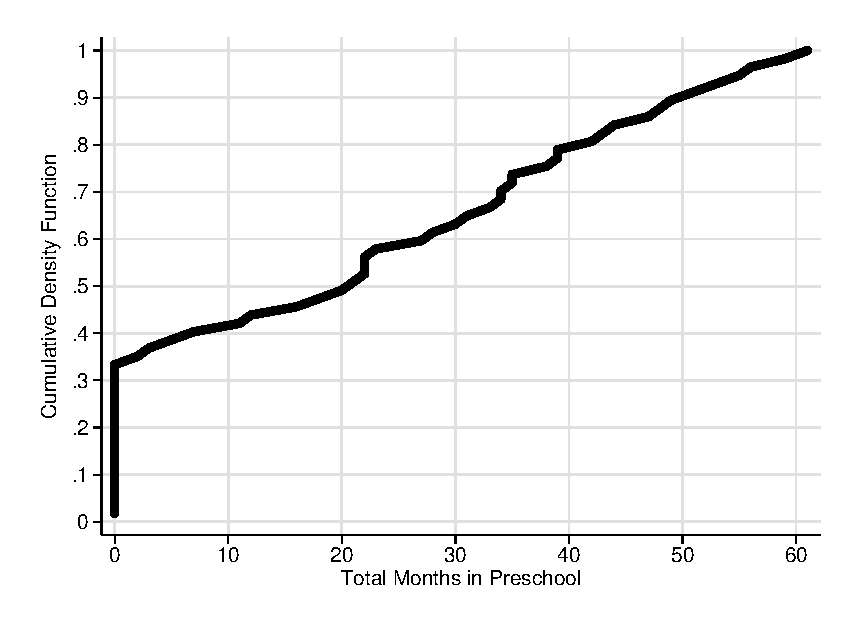
\includegraphics[width=.9\columnwidth]{output/abc_controlcontamination_months.eps}
\floatfoot{
\footnotesize
\noindent Note: This figure displays the cumulative density function of enrollment in alternative preschools of the control group in ABC.}
\end{figure}

\noindent In ABC, \treatsubsabc\ of control-group subjects were enrolled in one of 11 local center-based childcare centers (see Figure~\ref{fig:treatsubabc}). Most of these centers received federal subsidies and were therefore regulated by the Federal Interagency Day Care Requirements. Their staff members were required to be trained in early childhood education, and the centers were required to implement approved curricula designed to enhance cognitive, social, and linguistic competence in disadvantaged children. They had to comply to stringent staff-child ratios.\footnote{\citet{Burchinal_etal_1989_CD_Daycare-Pre-K-Dev}.} In CARE, \treatsubscarec\ of the control group and \treatsubscaref\ of the family education group were enrolled in alternative preschools by their parents (see Figure~\ref{fig:treatsubcare}). Parents in both of these groups had as options a similar set of local center-based childcare centers as the ABC children in the control group. We document this more thoroughly in Appendix~\ref{appendix:background}.

\begin{figure}[H]
		\caption{Control Substitution, CARE} \label{fig:treatsubcare}
		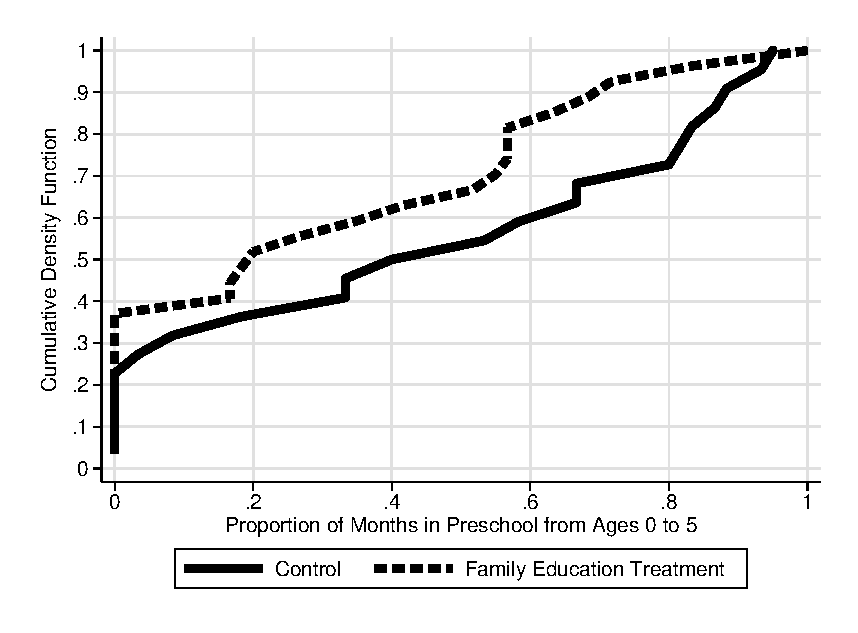
\includegraphics[width=.9\columnwidth]{output/care_controlcontamination_months.eps}
\floatfoot{
\footnotesize
\noindent Note: This figure displays the cumulative density function of enrollment in alternative preschools of the control and family education treatment groups in CARE.}
\end{figure}

\subsection{Program Costs}

\noindent The costs of the program are a fundamental input to our calculations of the benefit-to-cost ratio and the internal rate of return. We only perform these calculations for ABC due to data limitations---the documentation of the costs for  CARE is minimal. We provide a brief documentation of the costs of ABC next. In Appendix \ref{app:programcosts} we also explain other important components of the costs, including education, which is relevant given the substantial increase in long-term education for subjects of the treatment group. Similarly, it includes the costs of health and crime.\\


\noindent The program provided comprehensive center-based childcare and medical services. While we use some estimates from \cite{Masse_Barnett_2002_BOOKBenefitCostAnalysis}, our calculations of the program costs differ in two key aspects: (i) we account for the treatment group's medical care costs; and (ii) we incorporate new information on staff and program implementation to update costs. We calculate all costs as treatment effects; thus, costs of the program represent the costs of treatment minus the costs of the services that the control group received.\\

\begin{table}[H]
\begin{threeparttable}
\caption{Average Individual Costs, ABC} \label{tab:totalcosts}
\footnotesize
\begin{tabular}{ccccc|ccccc}\toprule
Year &\multicolumn{4}{c}{Treatment} &\multicolumn{4}{c}{Control} & Total \\ \midrule
& Medical$^{*}$ & Labor & Facilities & Other & Medical  & Labor & Facilities & Other& \\ \midrule
 1 	 & 	 \$888 	 & 	 \$11,895 	 & 	 \$5,700 	 & 	 \$1,053 	 & 	 \$888$^{*}$ 	 & 	 -   	 & 	 -   	 & 	 \$408 	 & 	 \$18,240 	 \\ 
 2 	 & 	 \$981 	 & 	 \$9,347 	 & 	 \$5,647 	 & 	 \$2,228 	 & 	 -   	 & 	 -   	 & 	 -   	 & 	 \$99 	 & 	 \$18,105 	 \\ 
 3 	 & 	 \$953 	 & 	 \$10,000 	 & 	 \$7,180 	 & 	 \$2,630 	 & 	 -   	 & 	 -   	 & 	 -   	 & 	 -   	 & 	 \$20,763 	 \\ 
 4 	 & 	 \$925 	 & 	 \$9,149 	 & 	 \$6,768 	 & 	 \$2,396 	 & 	 -   	 & 	 -   	 & 	 -   	 & 	 -   	 & 	 \$19,238 	 \\ 
 5 	 & 	 \$898 	 & 	 \$8,883 	 & 	 \$6,570 	 & 	 \$2,326 	 & 	 -   	 & 	 -   	 & 	 -   	 & 	 -   	 & 	 \$18,678 	 \\ \hline
 Total 	 & 	 \$4,645 	 & 	 \$49,275 	 & 	 \$31,865 	 & 	 \$10,634 	 & 	 \$888 	 & 	 -   	 & 	 -   	 & 	 \$507 	 & 	 \$95,024 	 \\
\bottomrule
\end{tabular}
\begin{tablenotes}
\footnotesize
\item Sources: See Appendix~\ref{app:programcosts}.\\
\item Note: This table summarizes the cost of the program by treatment and control group in 2014 USD, discounted to the year in which subjects were born. We consider only the rental rates of facilities and equipment. We include only the staff costs of staff who interacted with subjects directly or provided administrative support. $^{*}$The year 1 medical cost for the control group was only for the first cohort of ABC; the control groups of subsequent cohorts received no medical care. The change in costs between years 1, 2, 3, and years 4 and 5 reflect the change in childcare costs for infants and toddlers, and preschool-age children. The categories are described in the text below. Further details on each category of the table are provided in Appendix~\ref{app:programcosts}.
\end{tablenotes}
\end{threeparttable}
\end{table}


\noindent Table \ref{tab:totalcosts} shows the average costs per subject enrolled
in the program. It is important to note that we provide rental and marginal costs only, to capture, as closely as possible, the cost of replicating ABC.  For example, the costs do not include costs of research. The costs of the program are substantial and add up to \$95,024 for the average subject after discounting. This is the difference between the cost of goods and services provided to the treated subjects and the cost of those provided to the control subjects. \\

\subsection{Non-experimental Data Sources}

\noindent Our cost-benefit analysis requires (i) \textit{interpolation} of components we do not observe due to intermittent data collection; and (ii) \textit{extrapolation} or forecasting of components we do not observe because the follow-ups stop when the subjects were in their mid-30s. We use multiple sources of non-experimental data representative on the national or state level to construct these interpolations and extrapolations. Table~\ref{table:sources} details the components for which we do these exercises and the sources we use. Section~\ref{section:methodology} explains our methodology for doing so. 

\begin{table}[H]
\begin{threeparttable}
\caption{Auxiliary Data Sources for Interpolation and Extrapolation of Life-Cycle Benefits and Costs, ABC} \label{table:sources}
\footnotesize
%\input{../../AuxilliaryFiles/Preamble}
%\newgeometry{margin=.1in}

%\newcolumntype{L}[1]{>{\raggedright\let\newline\\\arraybackslash\hspace{0pt}}m{#1}}
%\newcolumntype{C}[1]{>{\centering\let\newline\\\arraybackslash\hspace{0pt}}m{#1}}
%\newcolumntype{R}[1]{>{\raggedleft\let\newline\\\arraybackslash\hspace{0pt}}m{#1}}

\begin{tabular}{L{3cm} C{1cm} C{1cm} C{1cm} C{1cm} C{1cm} C{2cm}} \toprule
 & \multicolumn{6}{c}{Subject's Age} \\
\textbf{Component}  & 16--21 & 21--30 & 31--34 & 34--50 & 61--67 & 68--Death \\ \midrule
\textbf{Transfer Income} & & \multicolumn{1}{c}{\cellcolor[gray]{.8} cNLSY} & \multicolumn{3}{c}{\cellcolor[gray]{.7} NLSY79; PSID}  &  \\ \midrule
\textbf{Subject Income} & &  \multicolumn{1}{c}{\cellcolor[gray]{.8} cNLSY} & \multicolumn{3}{c}{\cellcolor[gray]{.7} NLSY79; PSID} & \\ \midrule
\textbf{Health}  & \multicolumn{6}{c}{\cellcolor[gray]{.8} PSID; MEPS; MCBS; HRS}     \\ \midrule
\textbf{Crime} & \multicolumn{4}{c}{\cellcolor[gray]{.8} NCDPS; NJRP; NVS; UCRS} \\ \bottomrule
\end{tabular}
%\end{document}
\begin{tablenotes}
\footnotesize
Note: This table details the non-experimental data sources we use to interpolate and extrapolate the life-cycle benefits and costs of ABC. cNLSY: Children of the National Longitudinal Survey of the Youth 1979; NLSY79: National Longitudinal Survey of the Youth 1979; PSID: Panel Study of Income Dynamics; MEPS: Medical Expenditure Panel Survey; MCBS: Medicare Current Beneficiary Survey; HRS: Health and Retirement Study; NCDPS: North Carolina Department of Public Safety Data; NVS: National Crime Victimization Survey; NJRP: National Judicial Reporting Program; UCRS: Uniform Crime Reporting Statistics.
\end{tablenotes}
\end{threeparttable}
\end{table}

\section{Methodology} \label{section:methodology}

\subsection{Parameters of Interest and Policy Questions} \label{section:methodsquestions}

\noindent Random assignment to treatment alone does not guarantee that conventional treatment-effect estimates commonly used in the literature are able to answer policy-relevant questions. For an estimator to be useful in policy design, it should relate to a relevant parameter by clearly stating the counterfactual scenario to which the evaluated program is being compared. We define three parameters and link them to different policy questions.\\ 

\noindent Let $\Omega$ be a set with $\sigma$-algebra $\sigma \left( \Omega \right)$ characterizing the program's subjects, with generic element $\omega \in \Omega$. Let $Y$ denote an outcome of interest. $D$ indicates whether or not the parents of the subject agree to participate of the program and $R | D = 1$ denotes randomization to either treatment or control status; $T$ denotes the number of periods during the first phase of treatment---5 years.\footnote{We define parameters that are conditional on the parents agreeing to participate of the program. That is, conditional on $D = 1$. We find little sensitivity to the few cases of non-compliance in Appendix~\ref{appendix:assessingcc} and adjust our estimates for the cases of attrition as we explain in Appendix~\ref{appendix:attrition}.} We think of two counterfactuals under control status: 

\begin{eqnarray}
Y_H^0 \left( t, \omega \right) &:& \textbf{ Outcome under control status; subject stays at home in period $t$} \nonumber \\ 
Y_C^0 \left( t, \omega \right) &:& \textbf{ Outcome under control status; subject attends preschool in period $t$}  \nonumber
\end{eqnarray}

\noindent We define the proportion of months in alternative preschool as 

\begin{equation}
V \left ( \omega \right) : = \frac{\# \{ t: Y_H^0 \left( t, \omega \right) - Y_C^0 \left( t, \omega \right)  \} }{T}.
\end{equation}

\noindent Describing the dynamic choices underlying $V \left ( \omega \right)$ is of interest but goes beyond the scope of this paper. We simplify the analysis by assuming that 

\begin{align}
Y_H^0 \left( t, \omega \right) &= Y_H^0 \left( \omega \right) \nonumber \\
Y_C^0 \left( t, \omega \right) &= Y_C^0 \left( \omega \right).
\end{align}

\noindent We write the counterfactual outcome when the child is fixed to control status as 

\begin{equation}
Y^0 \left( \omega \right) : = \left[ 1 - V \left( \omega \right) \right] Y_H^0 \left( \omega \right) + \left[ V \left( \omega \right) \right] Y_C^0 \left( \omega \right), 
\end{equation}

\noindent and make explicit its dependence on $V \left( \omega \right)$, allowing us to answer policy-relevant questions.\\

\noindent There are two possible approaches. One approach is to treat $V \left( \omega \right)$ as binary, where $V \left( \omega \right) = 0$ or $V \left( \omega \right)  > 0$. The other approach is to allow for multiple values of $V$ and let $V$ to be continuous in the limit. The latter approach is ideal, because it would allow us to construct the counterfactual $Y_C^0 \left( v,  \omega \right) $ for $v \in [0 , 1]$ denoting a realization of $V$. This approach, however, is problematic in the context of the small number of observations in our experimental datasets. While the former approach limits the cases to either $V \left( \omega \right) = 0$ or $V \left( \omega \right)  > 0$, it still allows for the definition of policy-relevant parameters. Under this approach, we can frame the parental decision in a standard Roy-type setting noting that 

\begin{equation}
\Pr \left[ Y^1 \left( \omega \right) \geq \max \left(  Y_{H}^0 \left( \omega \right) ,  Y_{C}^0 \left( \omega \right)   \right) \right] = 1, \label{eq:noutility}
\end{equation}

\noindent where we could also frame the problem in terms of parental utility function $U \left( \cdot \right) $ over the outcome $Y$. We present estimates for different versions of this Roy model in Appendix~\ref{appendix:amethodology}.\\ 

\noindent We focus on simpler parameters that we can directly use in the cost-benefit analysis. The estimates of these parameters and the Roy-model equivalents are qualitatively similar. The first parameter of interest relates to the following question: what is the effect of the program as implemented? That is, what is the effect of the program without fixing the parental decision of whether or not to enroll the subject in alternative preschool? Importantly, this parameter does not speak to the effectiveness of the program by itself. Instead, it speaks to the effectiveness of the program relative to the supply of alternatives preschools that was in place when the program was implemented. The parameter is: 

\begin{equation}
\Delta := \mathbb{E}_{\Omega} \left[ Y^1 \left( \omega \right) -  \max \left(  Y_{H}^0 \left( \omega \right) ,  Y_{C}^0 \left( \omega \right)  \right) | D =1 \right]. \label{eq:mainest}
\end{equation}

\noindent Random assignment to either the treatment or control group allows us to identify this parameter.\\ 

\noindent It is perhaps more policy-relevant to inquire on the efficiency of a program with respect to a clearly stated counterfactual. For example, we want to ask: what is the effectiveness of the program with respect to a counterfactual in which the child stays at home? A parameter associated with that question is: 

\begin{equation}
\Delta \left( v = 0 \right) : =   \mathbb{E}_{\Omega} \left[ Y^1 \left( v, \omega \right) - Y^0 \left( v, \omega \right) | V = 0, D = 1 \right]. \label{eq:par0}
\end{equation}

\noindent Random assignment to the treatment group does not identify this parameter.\footnote{We abuse notation to index the realization of $V \left( \omega \right)$. Differently from the definition above, the first argument in $Y^r \left( \cdot, \cdot \right)$ represents the proportion of time in preschool alternatives and not a time period. We do this to avoid further complicating the indices of the counterfactual outcomes.} We can approximate it with the following estimator: 

\begin{equation}
\widehat{\Delta} \left( v = 0 \right) : = \widehat{\mathbf{E}} \left[ Y | R = 1, V \in \left[ 0 , \eta \right], D = 1 \right] - \widehat{\mathbf{E}} \left[ Y | R = 0, V \in \left[ 0 , \eta \right], D = 1 \right] \label{eq:estimates0}
\end{equation}

\noindent with $\eta \rightarrow 0$ and where $\widehat{\mathbf{E}}[\cdot]$ represents an estimate of $\mathbb{E}[\cdot]$. That is, we compare the subjects randomly assigned to treatment with the subjects randomly assigned to control in a neighborhood where subjects do not take preschool alternatives. Various matching estimators allow us to estimate how likely subjects are to take preschool alternatives, based on observed characteristics \citep{Heckman_Ichimura_etal_1997_REStud,Heckman_Ichimura_etal_1998_REStud}. We provide different versions of these estimators below.\\

\noindent Similarly, we define a parameter that allows us to compare the effectiveness of the program relative to the preschool alternatives: 

\begin{equation}
\Delta \left( v > 0 \right) : =   \mathbb{E}_{\Omega} \left[ Y^1 \left( v, \omega \right) - Y^0 \left( v, \omega \right) | V > 0, D = 1 \right] \label{eq:par1}
\end{equation}

\noindent and provide an estimate analogous to \eqref{eq:estimates0}. The parameters in \eqref{eq:par0} and \eqref{eq:par1} address control substitution, in the sense that they fix the counterfactual comparison accounting for the decisions that the parents make to enroll children in alternative preschools.

\subsection{Testing Multiple Hypotheses}  \label{section:counts}

\noindent We are interested in the effects that the program has on multiple dimensions of human development. We have measures of outcomes from very early in life to the mid-30s. This generates a multiple hypothesis testing problem. Two approaches are: (i) adjust the inference to account for the correlation of the outcomes using a step-down procedure \citep{Lehman_Romano_2005_AnnStat,Romano_Shaikh_2006_AnnStat}; and (ii) monetize the outcomes to produce a cost-benefit analysis. We adjust the inference when estimating the parameters in Section~\ref{section:methodsquestions} as in \citet{Lehman_Romano_2005_AnnStat} and \citet{Romano_Shaikh_2006_AnnStat} and provide a cost-benefit analysis below. In this section, we provide an intermediate alternative that informs on the relative importance of different outcomes in the cost-benefit analysis.\\

\noindent Let $\mathcal{G}$ be the index set for different groups of outcomes and let $\mathcal{O}_{g}$ be a group of outcomes, with $g \in \mathcal{G}$. Let $F_{j,g}^R \left( y_g^R\right) $ be the marginal distribution of outcome $j$ in group $g$ when randomized into treatment $R = 1$ or control $R = 0$. Assume that we want to perform inference on estimates of parameters of the type \eqref{eq:mainest} across multiple outcomes. That is, inference on 

\begin{equation}
\Delta_{j,g} := \mathbb{E}_{\Omega} \left[ Y_{j,g}^1 \left( \omega \right) -  \max \left(  Y_{j,g,H}^0 \left( \omega \right) ,  Y_{j,g,C}^0 \left( \omega \right)  \right) | D =1 \right]. 
\end{equation}

\noindent for the group of outcomes in $\mathcal{O}_{g}$. We want to test the null hypothesis 


\begin{equation}
H_{0} : F_{j,g}^0 = F_{j,g}^1, \ \forall \ j \in \mathcal{O}_{g}. 
\end{equation}

\noindent In practice, we test the hypothesis  

\begin{equation}
H_{0} : \Delta_{j,g} = 0, \ \forall \ j \in \mathcal{O}_{g}. 
\end{equation}

\noindent We use the following statistic to test this hypothesis: 

\begin{equation}
T_{g} = \sum _{j=1}^{\# \mathcal{O}_g} \mathbf{1} \left[ \widehat{\Delta}_{j}^{g} > 0\right]. \label{eq:count}
\end{equation} 

\noindent For inference purposes, we bootstrap this procedure and construct a null distribution. The $p$-value for the number of socially positive treatment effects in group $g$ is $1 - \widehat{F}_{g} \left( T_{g} \right)$, where $ \widehat{F}_{g}$ is the empirical bootstrap distribution of group $g$.\footnote{For the case where we count the number of positive and significant outcomes, we use a ``double bootstrap'' to produce an inference on the count. We resample $B_{0}$ times to obtain the $p$-value for testing the hypothesis of interest for each individual outcome. This allows us to compute the number of positive and significant treatment effects, for example. We repeat this procedure $B_{1}$ times to obtain a distribution for this count. Thus, the double bootstrap consists of $B_{0} \times B_{1}$ data resamplings.}\\

\noindent A particular case is to count the positive treatment effects in the outcomes across all the groups indexed in the set $\mathcal{G}$. This allows us to avoid (i) arbitrarily picking outcomes that have statistically significant effects---``cherry picking''; or (ii) arbitrarily blocking sets of outcomes to correct the $p$-values when accounting for multiple hypothesis testing.\\

\noindent We provide inference on this count and on a count of treatment effects that are both positive and significant for which the inference is analogous. We also provide counts for the parameters that account for control substitution.

\subsection{Forecasting and Monetizing Life-cycle Costs and Benefits} \label{section:cbamethodology}

\noindent In this section, we explain our strategy to interpolate and extrapolate the life-cycle costs and benefits of labor income, crime, and health. The methodology for doing this exercise for parental and public-transfer income is analogous to that of labor income so we suppress it for brevity. More methodological and practical details are in Appendix~\ref{appendix:methodology}, in which we also explain a solution for cases of attrition when producing interpolations and extrapolations. Based on our forecasts, we estimate the parameters in Section~\ref{section:methodsquestions} to perform the cost-benefit analysis of the program with and without accounting for control substitution.

\subsubsection{Labor Income}

\noindent We observe labor income at ages 21 and 30. To construct a life-cycle profile, we interpolate between ages 21 and 30 and extrapolate from ages 31 to 67, in which we assume that the subjects retire. For simplicity, we suppress $D$ and drop individual and time subscripts. Recall that $R$ indicates whether the subject was randomized to the treatment group ($R=1$) or to the control group ($R=0$), conditional on having agreed to participate in the program ($D = 1$). $Y$ is the outcome for which we want to produce a forecast---interpolation or extrapolation. In this case, the outcome is labor income. $X$ is a vector of observed characteristics, possibly affected by the treatment---e.g. lagged values of $Y$; $W$ is a vector of baseline characteristics---e.g. race and gender; $S$ indicates whether we observe $Y$ in ABC's experimental sample ($S=1$) or an auxiliary, non-experimental data source ($S=0$).\\

\noindent Our objective is to recover a forecast for $Y$ of the type

\begin{equation}
\widehat{Y} = \widehat{\phi} \left( R, X, W, S = 1 \right) + \widehat{\varepsilon},   \label{eq:additive}
\end{equation}

\noindent where $\phi \left( R, X, W, S \right) : = \mathbb{E} \left[ Y | R = r, X = x, W = w, S = s \right] $ and $\widehat{\varepsilon}$ is a forecasting error. That is, we assume that the outcome of interest is an additively separable function of the known objects $R, X, W, S$ and an unobserved component $\varepsilon$: 

\begin{assumption} (Additive Separability of the Outcome) \label{ass:additive}
\begin{equation}
Y = \phi \left( R, X, W, S \right) + \varepsilon. 
\end{equation}
\end{assumption}

\noindent Identifying $\phi \left( R, X, W, S \right)$ requires three assumptions. First, the forecast is based on observed characteristics, $X$. Thus, we require the auxiliary datasets to share the support on observed characteristics with the experimental dataset: 

\begin{assumption} \label{ass:support} (Common Support Between the Experimental and Auxiliary Datasets)
\begin{equation}
\sup \left( X | S = 1 \right) \subseteq \sup \left( X | S = 0 \right).
\end{equation}
\end{assumption}

\noindent Second, we assume that we are able to summarize the impacts that the treatment has on the outcomes with observed characteristics, given that we are not able to observe $R$ in the auxiliary dataset. Similarly, we need to be able to summarize the difference between the individuals in the experimental datasets and those in the auxiliary datasets based on observed characteristics. This is the third assumption. The second and third  assumptions are related, as they establish the requirements for being able to ``link'' the individuals in the auxiliary and experimental datasets when producing the forecasts. Formally, let $^{*}$ denote variables we do not observe. In the auxiliary dataset we have: $\left( S = 0, Y, X, W, R^* \right)$. In the experimental dataset we have: $\left( S = 1, Y^*, X, W, R \right)$. The second and third assumptions are:  

\begin{assumption} (Conditional Independence and Sufficiency of $S, X, W$ to Describe Treatment)
\begin{equation}
\mathbb{E} \left[ Y | R = r, X = x, W = w, S = s\right] =  \mathbb{E} \left[ Y | X = x^r, W = w, S = s\right]
\end{equation}

\noindent where $x^r$ is a draw from the distribution of $X | R = r$. 
\end{assumption}

\begin{assumption} (Conditional Independence and Sufficiency of $X, W, R$ to Describe Presence in a Dataset)
\begin{equation}
\mathbb{E} \left[ Y^* | R = r, X = x, W = w, S = 1 \right] = \mathbb{E} \left[ Y | R^* = r , X = x, W = w, S = 0\right]. 
\end{equation}
\end{assumption}

\noindent These three assumptions imply that 

\begin{equation}
\phi \left( R, X, W, S = 1 \right) = \mathbb{E} \left[ Y | X = x^r, W = w, S = 0 \right]  
\end{equation}

\noindent where $\mathbb{E} \left[ Y | X = x^r, W = w, S = 0 \right]$ is a moment in the auxiliary dataset. The estimation of $\mathbb{E} \left[ Y | X = x^r, W = w, S = 0 \right]$ produces a residual of the form $\widehat{\varepsilon} : = Y - \widehat{Y}$ for each individual. The forecast for each  individual outcome consists of $\widehat{\phi} \left( \cdot \right)$ and a draw from the empirical distribution of $\widehat{\varepsilon}$, which we call forecast error. We account for it when interpolating and extrapolating the crime and health outcomes in addition to income.

\subsubsection{Crime}  \label{sec:crime}

\noindent In this section, we explain how we quantify the benefits of the program from reductions in the subject's criminal activity. Two previous studies consider the impacts of ABC on crime: \citet{Clarke_Campbell_1998_ABC_Comparison_ECRQ} use administrative crime records up to age 21, and find no significant differences between the treatment and the control groups. \cite{Barnett_Masse_2007_EER} mention crime in their cost-benefit analysis, but they cite the previous study to claim that there are no savings coming from a reduction in crime. We consider richer data than the previous studies, which allows us to consider crime with a comprehensive life-cycle perspective: we gather various data sources, including administrative data on individual criminal records up to age 34, and project crimes until age 50 using prediction models based on local microdata. \\

\noindent We consider the following types of crime: arson, assault, burglary, fraud, larceny, miscellaneous (which includes traffic and non-violent drug crimes), murder, vehicle theft, rape, robbery, and vandalism. We use data from: (i) administrative youth arrests datasets, gathered for the age-21 follow-up; (ii) administrative adult arrests datasets, gathered around age 34; (iii) administrative sentences datasets, gathered around age 34; and (iv) self-reported adult crimes datasets, gathered in the age-21 and age-30 subject interviews. Because none of these data sources capture all criminal activity, it is necessary to combine them to more completely approximate the crimes the subjects committed. These datasets are discussed more extensively in Appendix \ref{appendix:crime}. The data are comprehensive and cover the full potential criminal career of subjects up to age 34, including details on the types of crimes and their timing, as well as projected and effective sentences. \\

\noindent We use several auxiliary datasets to construct national arrests-to-sentences and victims-to-arrests ratios: (i) the National Crime Victimization Survey (NCVS) to estimate the number of victims of crime; (ii) the National Judicial Reporting Program (NJRP) to estimate the number of sentences; and (iii) the Uniform Crime Reporting Statistics (UCRS) to estimate the number of arrests. Finally, we use microdata from the North Carolina Department of Public Safety (NCDPS) to estimate a prediction model for future crimes. This dataset contains information since 1972 on every individual who was convicted of a crime and entered the state prison system. \\

\noindent We follow four steps to estimate the costs of crime. We summarize the steps here and present a broader discussion in
Appendix \ref{appendix:crime}. \\

\begin{enumerate}
\item \textit{Count arrests and sentences.} We start by counting the total number of sentences for each individual
and type of crime (robbery, larceny, etc.) up to age 34. Then, we match the data on adult arrests, juvenile arrests, and self-reported crimes, to construct the total number of  arrests for each individual and type of crime up to that age.\footnote{In practice, we count all offenses (an arrest might include multiple offenses). This gives the correct number of victims for our estimations. The youth data have coarser categories than the rest of the data, so we assume that all property crimes were larcenies and that all violent crimes are assaults. In our sample, assault is the most common type of violent crime, and larceny/theft is the most common property crime.} About 10\% of the ABC sample has missing arrest data. For these cases, we impute the number of arrests by multiplying the number of sentences for each type of crime by the  national arrests-to-sentences ratio for the respective crime.

\item \textit{Construct predictions.} Based on the sentences observed before age 34, we predict the sentences
that the ABC subjects will have after that age. The NCDPS data provide lifetime sentences of individuals in North Carolina, the same state in which the program was implemented. In that dataset, we estimate linear prediction models for each type of crime in which sentences after age 34 are the outcomes, and sentences up to age 34 are the regressors. Then, we apply these models to the ABC data. The outcome for each crime type is the number of future sentences for each subject, up to age 50. We assume that individuals with no criminal records before age 34 commit no crimes after age 34. We then add these estimates to the original number of sentences, getting an estimate of the lifetime sentences. To the best of our knowledge, no prior study on the benefits and costs of an educational program has used microdata to estimate a predictive model for future crimes. The predictions are an important component of total crime, as adding them increases the total count of crimes by 30\%--50\%. The prediction models we estimate and the results in terms of additional crimes are presented in Appendix \ref{appendix:crime}.

\item \textit{Estimate number of victims of crimes.} We observe crimes that resulted in consequences in the judicial system (i.e. crimes that resulted in arrests, sentences, or both). However, it is possible that for any subject for whom we observe to have committed a crime, he committed more crimes that we do not observe. Victimization inflation (VI) is a method to capture benefits of crime reduction for crimes without consequences in the judicial system that are unobserved in the ABC data. Previous papers using this method include \citet{Belfield_Nores_etal_2006_JHR} and \cite{Heckman_Moon_etal_2010_RateofReturn}. We start by constructing a VI ratio, which is the national ratio of victims-to-arrests for each type of crime.\footnote{We assume that each crime with victims is counted separately in the national reports on arrests, even for arrests that might have been motivated by more than one crime.} Then, we estimate the number of victims for each type of crime committed by ABC subjects as their total arrests multiplied by the VI ratio. Additionally, we can calculate an analogous estimate of the number of crime victims using sentences, based on the VI ratio and the national arrests-to-sentences ratio. Both estimates are very similar, as shown in Appendix \ref{appendix:crime}. To improve precision, the estimates in the rest of our paper are based on the average of the two.

\item \textit{Find total costs of crimes.} We use the estimates of the cost of crimes for victims from \cite{McCollister_etal_2010_DAD} to impute the total victimization costs (see Appendix \ref{appendix:crime} for details on the costs we use). For crimes having arrests, sentences, or both, we consider judicial system costs as well, such as police costs.\footnote{To be able to assign costs to each type of crime, we assume that the cost of the justice system depends on the number of offenses of each type, rather than on the number of arrests. While this could very slightly overestimate justice system costs, the costs only represent about 5\% of the total crime costs.} Finally, we construct the total costs of incarceration for each subject using the total prison time and the cost of a day in prison.
\end{enumerate}

\subsubsection{Health} \label{section:health}

\noindent We use an alternative methodology for health-related outcomes. There are three main reasons for this: (i) health outcomes such as diabetes or heart disease are absorbing states; (ii) health outcomes are highly interdependent within and across time; and (iii) there is no evident time period available to finish accounting for benefits and costs. For example, for income we extrapolate up to the retirement age of 67. However, for health, we need to predict an age of death for each individual. Thus, using the notation so far, it is not sufficient to condition on $W, Z, X$ to recover a credible estimate of the treatment effect. Instead, we use an adaptation of the Future America Model (FAM) that projects health outcomes from the age of the supplemental health follow-up during the mid-30s up to the projected death of the individuals \citep{Goldman_etal_2015_Future-Elderly-Model-Report}. \\

\noindent We provide a brief description of the model in this subsection. Appendix~\ref{appendix:health} provides a thorough discussion. The methodology has five steps: (i) estimate the age-by-age health state transition probabilities using the Panel Study of Income Dynamics (PSID); (ii) match these transition probabilities to the ABC individuals based on observed characteristics; (iii) estimate quality-adjusted life year (QALY) models using the Medical Expenditure Panel Survey (MEPS) and the PSID; (iv) estimate medical cost models using the MEPS and the Medicare Current Beneficiary Survey (MCBS), allowing estimates to differ by health state and observed characteristics; and (v) predict the medical expenditure and QALYs that correspond to the simulated individual health trajectories. \\

\noindent Our microsimulation model starts the health predictions at age 30, with the information on observed characteristics available at this age. We restrict it to the individuals for whom we have information from the age-34 health follow-up. This allows us to account for components that are crucial for predicting health outcomes, such as the body mass index (BMI). The models predict the probability of being in any of the states in the horizontal axis of Table~\ref{table:transition} at age $a+1$ based on the state at age $a$, which is described by the vertical axis of the table. The crosses indicate if the estimation of the probability of being in a state at age $a$ is relevant for the state at age $a + 1$. Absorbing states are an exception. For example, heart disease at age $a$ does not enter in the estimation of transitions for heart disease at age $a+1$ because it is an absorbing state: once a person has heart disease, she carries it through the rest of her life. The same is true for chronic or permanent conditions such as hypertension, having a stroke, etc.

\begin{sidewaystable}[H]
\begin{threeparttable}
\caption{Health State Transitions, Age $a$ as Predictor of Age $a+1$}\label{table:transition}
\scriptsize
\begin{tabular}{l|cccccccccccccc} \toprule
\multicolumn{1}{c}{Age $a$} & \multicolumn{14}{c}{Age $a+1$} \\ \midrule
  & Heart & Hyper- & Stroke & Lung  & Diabetes & Cancer & Disability & Mortality & Smoking  & Obesity & Health  & DI  & SS  & SSI  \\
&  Disease & tension &  & Disease & & & & &  &  & Insurance & Claim & Claim & Claim \\
Heart Disease & & & $\times$& & & &$\times$ &$\times$ & $\times$           &       &  $\times$  & $\times$ & $\times$ & $\times$\\
Hypertension  &  $\times$& & $\times$ & & & &$\times$ &$\times$ &       &     & $\times$   & $\times$ & $\times$  & $\times$\\
Stroke           & & & & & & &$\times$ &$\times$ &             &      &   $\times$  & $\times$ & $\times$  & $\times$\\
Lung Disease & & & & & & &$\times$ &$\times$ & $\times$         &        &   $\times$  &$\times$  & $\times$  & $\times$\\
Diabetes       & $\times$ &$\times$  & $\times$   & & & &$\times$ &$\times$ & $\times$            &       &  $\times$    & $\times$& $\times$ & $\times$ \\
Cancer         & & & $\times$ &  & &   &$\times$ & $\times$&           &         &   $\times$  & $\times$ & $\times$  & $\times$\\
Disability     & & & & & & &$\times$ &$\times$ &         &      &     $\times$  & $\times$ & $\times$   & $\times$\\
\midrule
Smoking & $\times$& $\times$&$\times$ & $\times$& $\times$& $\times$&$\times$ &$\times$ & $\times$   &   &     $\times$  & $\times$ & $\times$   & $\times$\\
BMI & $\times$& $\times$&$\times$ & $\times$& $\times$& $\times$&$\times$ & & $\times$    &  $\times$ &     &  &   & \\
Physical Activ. & $\times$& $\times$&$\times$ & $\times$& $\times$& $\times$&$\times$ & & $\times$    &   &     &   &  & \\
Binge Drinking & & & & & & &  &$\times$ & $\times$    &      &      &   &     &  \\
\midrule
DI Claim      & & & & &  & & & &             &         & $\times$    & $\times$   & $\times$ & $\times$\\
SS Claim     & & & & & & & &           &         &     & $\times$ &  & & $\times$\\
SSI Claim   & & & & &&  & & &         &        &      & &   & $\times$\\ \bottomrule
\end{tabular}

\begin{tablenotes}
\footnotesize
\item Note: This table illustrates how health outcomes at age $a$ predict health outcomes at age $a+1$. The crosses indicate if we use the age $a$ outcome to predict the age $a+1$ outcome. DI Claim: disability insurance claim; SS Claim: social security claim; DB Claim: disability benefits claim; SSI Claim: supplemental security income claim. The age $a$ states that do not predict themselves at age $a+1$ are absorbing states by construction.
\end{tablenotes}
\end{threeparttable}
\end{sidewaystable}

\noindent At each age, once we obtain the transition probability for each health outcome, we draw $5,000$ Monte-Carlo simulations for each subject. Thus, each simulation depends on each individual's health history and on their particular characteristics. For every simulated trajectory of health outcomes, we are able to predict the lifetime medical expenditure using the models estimated from the MEPS and the MCBS. We are then able to obtain an estimate of the expected lifetime medical expenditure for every subject in our primary sample by taking the mean of each individual's simulated lifetime medical expenditure. The same procedure is applied to QALYs. This estimate is used as the dependent variable in our linear regressions for calculating treatment effects on health costs. \\

\noindent A quality-adjusted life year (QALY) reweighs a year of life according to its quality given the burden of disease. A QALY of 1 denotes a year of life in the absence of disease (perfect health). The value of QALY for an individual in a given year is smaller than 1 when there is positive burden of disease, as worse health conditions imply lower QALYs.\footnote{When an individual dies, her QALY equals zero. It is worth noting that there are extreme combinations of disease and disability that may generate negative QALYs, although this case is unusual.} We compute a QALY model based on the EQ-5D instrument, a widely-used Health-related Quality-of-life (HRQoL) measure, available in MEPS. We then estimate this model from the PSID. Appendix~\ref{appendix:health} provides more details on this estimation strategy. \\

\noindent We estimate four models of medical spending: total medical spending (medical spending from all payment sources), Medicare spending (annual medical spending paid by parts A, B, and D of Medicare), Medicaid spending (medical spending paid by Medicaid), and out-of-pocket spending (medical spending paid directly by the individual). Each medical spending model is estimated through pooled weighted least squares regressions that include a person's demographics, economic status, current health, lagged health, risk factors, and functional status as explanatory variables. For the estimation of medical spending corresponding to non-Medicare eligible individuals we use the MEPS, and for Medicare-eligible individuals we use the MCBS.\\ 

\noindent \textbf{Medical Expenditure before Age 30}

\noindent We combine the MEPS and retrospective information in the ABC interviews at ages 21 and 30 related to hospitalizations at ages 12 and 15 and births at age 15. In addition to this retrospective information, we use use individual and family demographics to predict medical expenditure models for each age, as summarized in Table~\ref{table:pre30}.\\

\begin{table}[H]
\begin{threeparttable}
\caption{Health Expenditure Models by Age Group, before Age 30}\label{table:pre30}
\begin{tabular}{lcccc} \toprule
Explanatory variable & \multicolumn{4}{c}{Age Group} \\
& 8-11 & 12-14 & 15-20 & 21-30 \\
\midrule
Race/ethnicity & \checkmark & \checkmark & \checkmark & \checkmark \\
Hospital stays & if $\geq$ 1 week & any stay & \# nights & $\times$ \\
Births & $\times$ & $\times$ & \checkmark & \checkmark \\
Mother present & $\times$ & \checkmark & \checkmark & $\times$ \\
Father present & \checkmark & \checkmark & $\times$ & $\times$ \\
Number of siblings & \checkmark & \checkmark & $\times$ & $\times$ \\
Foodstamps & \checkmark & \checkmark & \checkmark & \checkmark \\
Living arrangements & $\times$ & $\times$ & \checkmark & \checkmark \\
Working, if working age & \checkmark & \checkmark & \checkmark & \checkmark \\
\bottomrule
\end{tabular}
\begin{tablenotes}
\footnotesize
\item Note: This table summarizes the explanatory variables included in the models we use to predict medical expenditure for each age group. Possible living arrangements are: living with parents, away at college, married, or other.\\
\end{tablenotes}
\end{threeparttable}
\end{table}

\noindent The first level of each model predicts the likelihood that the subject incurred any medical expenditure in the period. The second level predicts the medical expenditure for those with positive expenditures.

\section{Results} \label{section:results}

\subsection{Treatment Effects} \label{section:teresults}

\noindent We consider \noutcomes\ measures of human development across the life cycle and count the measures for which the program had a ``socially positive'' effect, without accounting for control substitution. We do this for both ABC and CARE by focusing on the first phase of treatment to compare subjects who received center-based childcare to subjects who did not---noting that assignment was random.\footnote{In ABC, this implies comparing the subjects who were randomly assigned to the treatment group to the subjects who were randomly assigned to the control group, in the first phase. In CARE, this implies comparing the subjects who were randomly assigned to receive center-based childcare and family education to the subjects who were randomly assigned either to the group receiving family education only or to the control group, in the first phase as well.} Figure~\ref{fig:ppositive} displays the results from this exercise: ABC and CARE positively impact a large percentage of the outcomes we consider.\footnote{The calculation of the standard errors follows from the bootstrap procedure we discuss in Section~\ref{section:methodology}.}\\ 

\noindent We can further decompose the counts in Figure~\ref{fig:ppositive} into arbitrary categories. To economize space, we present this exercise pooling ABC and CARE. That is, we decompose the effects described in the last two bars of Figure~\ref{fig:ppositive}. Figure~\ref{fig:ppositivecategory1} and Figure~\ref{fig:ppositivecategory2} present this exercise. This helps us better understand the type of outcomes the programs affected. The results indicate that a large and precise fraction of effects are positive for outcomes spanning the life cycle, from parental income to crime and including a wide variety of health categories.\\ 

\noindent Next we present an overview of outcome-specific results. Appendix~\ref{appendix:results} displays an extensive summary of the estimates for the \noutcomes\ outcomes we consider. Note that: (i) we arbitrarily pick the outcomes we discuss next because we consider them of economic interest; and (ii) Appendix~\ref{appendix:results} displays results accounting for multiple hypothesis testing as in \citet{Lehman_Romano_2005_AnnStat} and \citet{Romano_Shaikh_2006_AnnStat}. We do not lose significance in the majority of outcomes.

\begin{figure}[H]
		\caption{Positively Impacted Outcomes, ABC and CARE} \label{fig:ppositive}
		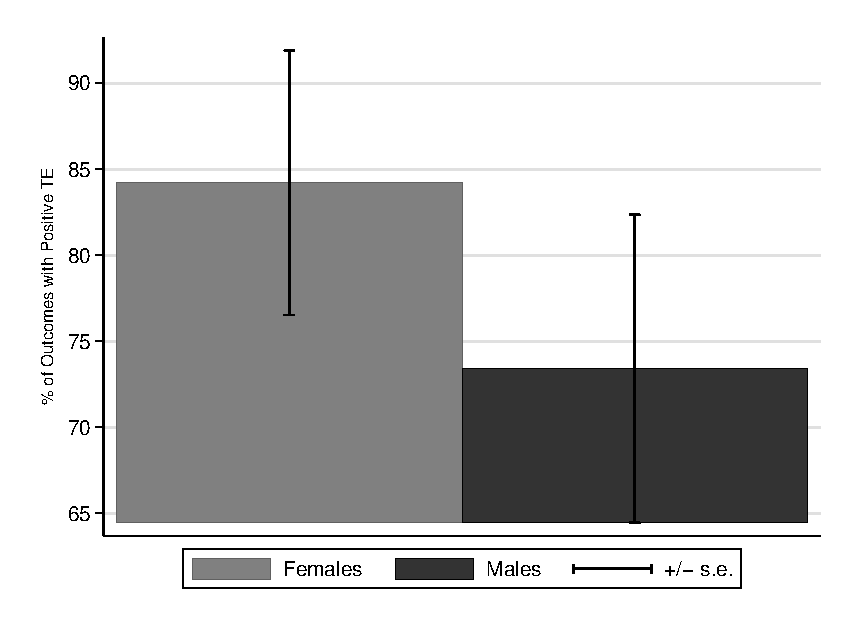
\includegraphics[width=.8\columnwidth]{output/itt_noctrl_all.eps}
\floatfoot{
\footnotesize
\noindent Note: The first two bars (ABC) compare the treatment and control groups in ABC. The third and fourth bars (CARE) compare the subjects who received center-based childcare and family education to the subjects who receive either family education or no treatment at all. The last two bars (ABC and CARE) pool the two previous sets of comparisons.}
\end{figure}

\noindent Table~\ref{table:females} presents the results for females. We focus on three columns. Columns~(2) displays the estimates of the parameter in \eqref{eq:mainest}. This parameter speaks to the effectiveness of the programs, \textit{as implemented}. Columns~(5) and ~(8) display estimates of the parameters in \eqref{eq:par0} and \eqref{eq:par1}. The former speaks to the effectiveness of the programs relative to the counterfactual of \textit{staying at home}. The latter speaks to the effectiveness of the programs relative to \textit{attending an alternative preschool}. All of these three estimates account for program attrition and control for a set of background variables.\footnote{See Appendix~\ref{appendix:methodology} for our methodology to account for attrition and Appendix~\ref{appendix:controls} for our procedure for selecting controls.}\\

\begin{figure}[H]
		\caption{Positively Impacted Outcomes by Category, ABC and CARE} \label{fig:ppositivecategory1}
		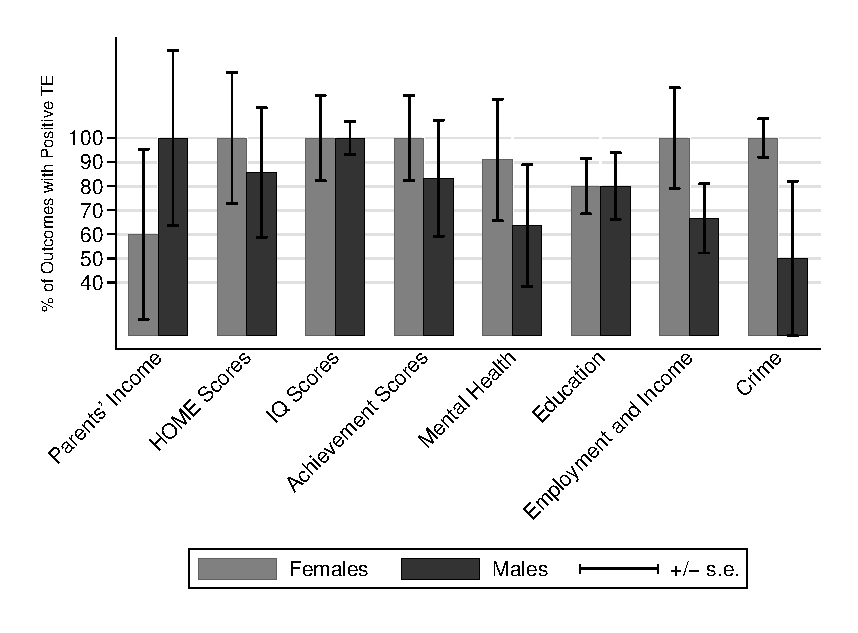
\includegraphics[width=.8\columnwidth]{output/itt_noctrl_cats1.eps}
\floatfoot{
\footnotesize
\noindent Note: For each outcome category, we compare the mean of the subjects who received center-based childcare in ABC and center-based childcare and family education in CARE to the mean of the subjects in the control group in ABC and the control group and the family education treatment group in CARE and count the number of positive comparisons.}
\end{figure}

\noindent Column~(2) shows that the program caused substantial gains in a variety of economically relevant short- and long-term outcomes, as implemented. First, the programs have an effect on IQ that goes beyond the effects of many early childhood education programs, which usually fade out after a year of elementary school \citep{Hojman_2015_EvidenceFadeOut,Elango_Hojman_etal_2016_Early-Edu}. To put this effect in perspective, note that IQ and achievement tests scores are standardized to a nationally representative population with a standard deviation of 15 points. The effect of the programs we study amounts to more than $2/3$ of a standard deviation. The largest effect of Head Start, for example, happens before elementary school and amounts to half of the effect of ABC at age 12, the latter effect being measured after elementary school \citep{Elango_Hojman_etal_2016_Early-Edu}. The programs also have a substantial effect on achievement, which not only measures cognition but mathematics and reading knowledge.

\begin{figure}[H]
		\caption{Positively Impacted Health Outcomes, ABC and CARE} \label{fig:ppositivecategory2}
		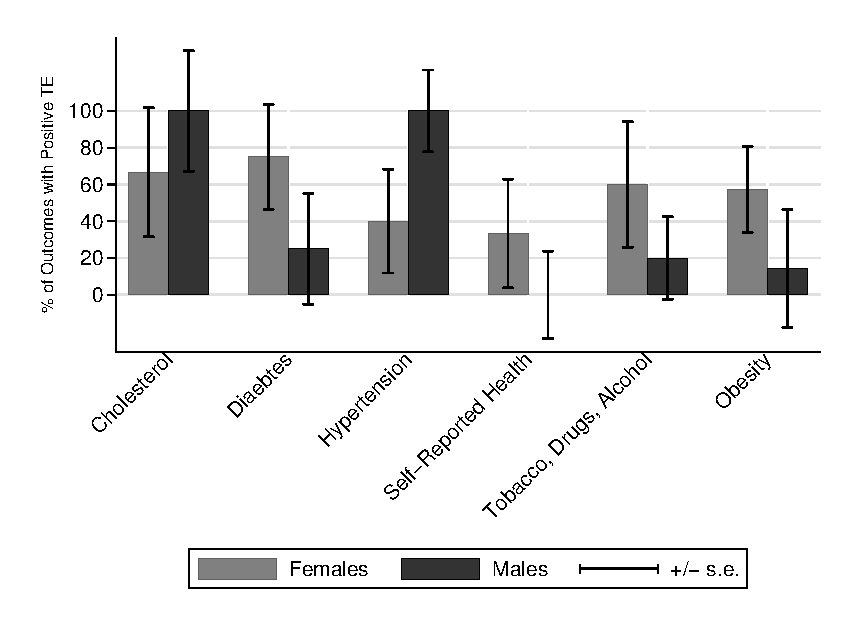
\includegraphics[width=.8\columnwidth]{output/itt_noctrl_cats2.eps}
\floatfoot{
\footnotesize
\noindent Note: For each outcome category, we compare the mean of the subjects who received center-based childcare in ABC and center-based childcare and family education in CARE to the mean of the subjects in the control group in ABC and the control group and the family education treatment group in CARE and count the number of positive comparisons.}
\end{figure} 

\noindent The effects that the programs have on high-school graduation and years of education at age 30 are sizable---column~(2). The former increases by \hsgradf\ percentage points and the latter by more than \yearsedf\ years. Although marginally not significant, the programs also: (i) increase labor income; (ii) reduce the dependence on public-transfer income; and (iii) increase employment. When we group the education and employment outcomes across ages 21 and 30 all of them display a positive treatment effect (see Figure~\ref{fig:ppositivecategory1}).\\

\noindent When fixing the counterfactuals, a clear pattern emerges: females benefit much more from the programs relative to staying at home compared to how they benefit from the programs relative to attending alternative preschools. The differences are substantial: more than $30$ percentage points in high school graduation, almost a year of education, around $\$ 3,000$ 2014 USD of labor income, among other examples. \\

\begin{table}[H] 
\begin{threeparttable}
\caption{Treatment Effects on Selected Outcomes, Females}
\label{table:females}
\centering
\scalebox{.97}{
\begin{table}[H]
\captionsetup{singlelinecheck=false,justification=centering}
\caption{ABC/CARE Average Treatment Effects, Females \\ Education, Employment, and Crime \label{tab:ate_female_main1}}

  \begin{threeparttable}
  \begin{tabular}{cccccccccc}
  \hline\hline

     &  & \scriptsize{(1)} & \scriptsize{(2)} & \scriptsize{(3)} & \scriptsize{(4)} & \scriptsize{(5)} & \scriptsize{(6)} & \scriptsize{(7)} & \scriptsize{(8)} \\  

     &  &  &  & \mc{3}{c}{\scriptsize{$P=0$}} & \mc{3}{c}{\scriptsize{$P=1$}} \\ 
    \cmidrule(lr){5-7} \cmidrule(lr){8-10} 

    \scriptsize{Variable} & \scriptsize{Age} & \scriptsize{ITT} & \scriptsize{ITT$|X,W$} & \scriptsize{ITT} & \scriptsize{ITT$|X,W$} & \scriptsize{KE$|X,W$} & \scriptsize{ITT} & \scriptsize{ITT$|X,W$} & \scriptsize{KE$|X,W$} \\ 
    \hline  

    \mc{1}{l}{\scriptsize{Std. IQ Test}} & \mc{1}{c}{\scriptsize{12}} & \mc{1}{c}{\scriptsize{8.259}} & \mc{1}{c}{\scriptsize{10.271}} & \mc{1}{c}{\scriptsize{8.457}} & \mc{1}{c}{\scriptsize{11.647}} & \mc{1}{c}{\scriptsize{7.881}} & \mc{1}{c}{\scriptsize{8.167}} & \mc{1}{c}{\scriptsize{9.877}} & \mc{1}{c}{\scriptsize{7.186}} \\  

     &  & \mc{1}{c}{\scriptsize{\textbf{(0.000)}}} & \mc{1}{c}{\scriptsize{\textbf{(0.000)}}} & \mc{1}{c}{\scriptsize{\textbf{(0.000)}}} & \mc{1}{c}{\scriptsize{\textbf{(0.020)}}} & \mc{1}{c}{\scriptsize{\textbf{(0.000)}}} & \mc{1}{c}{\scriptsize{\textbf{(0.000)}}} & \mc{1}{c}{\scriptsize{\textbf{(0.000)}}} & \mc{1}{c}{\scriptsize{\textbf{(0.020)}}} \\  

    \mc{1}{l}{\scriptsize{Std. Achv.  Test}} & \mc{1}{c}{\scriptsize{8}} & \mc{1}{c}{\scriptsize{5.404}} & \mc{1}{c}{\scriptsize{8.690}} & \mc{1}{c}{\scriptsize{8.100}} & \mc{1}{c}{\scriptsize{15.721}} & \mc{1}{c}{\scriptsize{11.046}} & \mc{1}{c}{\scriptsize{4.382}} & \mc{1}{c}{\scriptsize{7.048}} & \mc{1}{c}{\scriptsize{5.065}} \\  

     &  & \mc{1}{c}{\scriptsize{\textbf{(0.020)}}} & \mc{1}{c}{\scriptsize{\textbf{(0.000)}}} & \mc{1}{c}{\scriptsize{\textbf{(0.020)}}} & \mc{1}{c}{\scriptsize{\textbf{(0.000)}}} & \mc{1}{c}{\scriptsize{\textbf{(0.000)}}} & \mc{1}{c}{\scriptsize{\textbf{(0.059)}}} & \mc{1}{c}{\scriptsize{\textbf{(0.000)}}} & \mc{1}{c}{\scriptsize{\textbf{(0.020)}}} \\  

    \mc{1}{l}{\scriptsize{Graduated High School}} & \mc{1}{c}{\scriptsize{30}} & \mc{1}{c}{\scriptsize{0.213}} & \mc{1}{c}{\scriptsize{0.224}} & \mc{1}{c}{\scriptsize{0.367}} & \mc{1}{c}{\scriptsize{0.411}} & \mc{1}{c}{\scriptsize{0.352}} & \mc{1}{c}{\scriptsize{0.142}} & \mc{1}{c}{\scriptsize{0.146}} & \mc{1}{c}{\scriptsize{0.090}} \\  

     &  & \mc{1}{c}{\scriptsize{\textbf{(0.039)}}} & \mc{1}{c}{\scriptsize{\textbf{(0.039)}}} & \mc{1}{c}{\scriptsize{\textbf{(0.000)}}} & \mc{1}{c}{\scriptsize{\textbf{(0.000)}}} & \mc{1}{c}{\scriptsize{\textbf{(0.020)}}} & \mc{1}{c}{\scriptsize{(0.118)}} & \mc{1}{c}{\scriptsize{\textbf{(0.098)}}} & \mc{1}{c}{\scriptsize{(0.196)}} \\  

    \mc{1}{l}{\scriptsize{Years of Edu.}} & \mc{1}{c}{\scriptsize{30}} & \mc{1}{c}{\scriptsize{1.474}} & \mc{1}{c}{\scriptsize{1.696}} & \mc{1}{c}{\scriptsize{1.967}} & \mc{1}{c}{\scriptsize{2.247}} & \mc{1}{c}{\scriptsize{1.291}} & \mc{1}{c}{\scriptsize{1.244}} & \mc{1}{c}{\scriptsize{1.357}} & \mc{1}{c}{\scriptsize{0.993}} \\  

     &  & \mc{1}{c}{\scriptsize{\textbf{(0.020)}}} & \mc{1}{c}{\scriptsize{\textbf{(0.020)}}} & \mc{1}{c}{\scriptsize{\textbf{(0.020)}}} & \mc{1}{c}{\scriptsize{\textbf{(0.020)}}} & \mc{1}{c}{\scriptsize{(0.118)}} & \mc{1}{c}{\scriptsize{\textbf{(0.020)}}} & \mc{1}{c}{\scriptsize{\textbf{(0.020)}}} & \mc{1}{c}{\scriptsize{\textbf{(0.078)}}} \\  

    \mc{1}{l}{\scriptsize{Labor Income}} & \mc{1}{c}{\scriptsize{30}} & \mc{1}{c}{\scriptsize{928}} & \mc{1}{c}{\scriptsize{677}} & \mc{1}{c}{\scriptsize{1,433}} & \mc{1}{c}{\scriptsize{637}} & \mc{1}{c}{\scriptsize{1,391}} & \mc{1}{c}{\scriptsize{691}} & \mc{1}{c}{\scriptsize{308}} & \mc{1}{c}{\scriptsize{300}} \\  

     &  & \mc{1}{c}{\scriptsize{(0.314)}} & \mc{1}{c}{\scriptsize{(0.412)}} & \mc{1}{c}{\scriptsize{(0.353)}} & \mc{1}{c}{\scriptsize{(0.471)}} & \mc{1}{c}{\scriptsize{(0.235)}} & \mc{1}{c}{\scriptsize{(0.392)}} & \mc{1}{c}{\scriptsize{(0.392)}} & \mc{1}{c}{\scriptsize{(0.451)}} \\  

    \mc{1}{l}{\scriptsize{Public-Transfer Income}} & \mc{1}{c}{\scriptsize{30}} & \mc{1}{c}{\scriptsize{-884}} & \mc{1}{c}{\scriptsize{-951}} & \mc{1}{c}{\scriptsize{-980}} & \mc{1}{c}{\scriptsize{-971}} & \mc{1}{c}{\scriptsize{-508}} & \mc{1}{c}{\scriptsize{-839}} & \mc{1}{c}{\scriptsize{-964}} & \mc{1}{c}{\scriptsize{-676}} \\  

     &  & \mc{1}{c}{\scriptsize{\textbf{(0.059)}}} & \mc{1}{c}{\scriptsize{\textbf{(0.098)}}} & \mc{1}{c}{\scriptsize{\textbf{(0.020)}}} & \mc{1}{c}{\scriptsize{\textbf{(0.098)}}} & \mc{1}{c}{\scriptsize{(0.216)}} & \mc{1}{c}{\scriptsize{(0.118)}} & \mc{1}{c}{\scriptsize{(0.118)}} & \mc{1}{c}{\scriptsize{(0.157)}} \\  

    \mc{1}{l}{\scriptsize{Employed}} & \mc{1}{c}{\scriptsize{30}} & \mc{1}{c}{\scriptsize{0.110}} & \mc{1}{c}{\scriptsize{0.111}} & \mc{1}{c}{\scriptsize{0.233}} & \mc{1}{c}{\scriptsize{0.235}} & \mc{1}{c}{\scriptsize{0.204}} & \mc{1}{c}{\scriptsize{0.052}} & \mc{1}{c}{\scriptsize{0.056}} & \mc{1}{c}{\scriptsize{0.037}} \\  

     &  & \mc{1}{c}{\scriptsize{\textbf{(0.078)}}} & \mc{1}{c}{\scriptsize{\textbf{(0.098)}}} & \mc{1}{c}{\scriptsize{\textbf{(0.000)}}} & \mc{1}{c}{\scriptsize{\textbf{(0.078)}}} & \mc{1}{c}{\scriptsize{(0.157)}} & \mc{1}{c}{\scriptsize{(0.314)}} & \mc{1}{c}{\scriptsize{(0.255)}} & \mc{1}{c}{\scriptsize{(0.373)}} \\  

    \mc{1}{l}{\scriptsize{Total Felony Arrests}} & \mc{1}{c}{\scriptsize{Mid-30s}} & \mc{1}{c}{\scriptsize{-0.266}} & \mc{1}{c}{\scriptsize{-0.337}} & \mc{1}{c}{\scriptsize{-0.763}} & \mc{1}{c}{\scriptsize{-1.004}} & \mc{1}{c}{\scriptsize{-1.046}} & \mc{1}{c}{\scriptsize{-0.050}} & \mc{1}{c}{\scriptsize{-0.078}} & \mc{1}{c}{\scriptsize{-0.021}} \\  

     &  & \mc{1}{c}{\scriptsize{(0.157)}} & \mc{1}{c}{\scriptsize{(0.137)}} & \mc{1}{c}{\scriptsize{\textbf{(0.098)}}} & \mc{1}{c}{\scriptsize{(0.137)}} & \mc{1}{c}{\scriptsize{(0.118)}} & \mc{1}{c}{\scriptsize{(0.255)}} & \mc{1}{c}{\scriptsize{(0.196)}} & \mc{1}{c}{\scriptsize{(0.392)}} \\  

    \mc{1}{l}{\scriptsize{Total Misdemeanor Arrests}} & \mc{1}{c}{\scriptsize{Mid-30s}} & \mc{1}{c}{\scriptsize{-0.918}} & \mc{1}{c}{\scriptsize{-1.081}} & \mc{1}{c}{\scriptsize{-1.939}} & \mc{1}{c}{\scriptsize{-2.437}} & \mc{1}{c}{\scriptsize{-2.284}} & \mc{1}{c}{\scriptsize{-0.475}} & \mc{1}{c}{\scriptsize{-0.556}} & \mc{1}{c}{\scriptsize{-0.224}} \\  

     &  & \mc{1}{c}{\scriptsize{\textbf{(0.020)}}} & \mc{1}{c}{\scriptsize{\textbf{(0.078)}}} & \mc{1}{c}{\scriptsize{\textbf{(0.059)}}} & \mc{1}{c}{\scriptsize{\textbf{(0.078)}}} & \mc{1}{c}{\scriptsize{\textbf{(0.000)}}} & \mc{1}{c}{\scriptsize{(0.137)}} & \mc{1}{c}{\scriptsize{(0.118)}} & \mc{1}{c}{\scriptsize{(0.196)}} \\  

    \mc{1}{l}{\scriptsize{Total Years Incarcerated}} & \mc{1}{c}{\scriptsize{30}} & \mc{1}{c}{\scriptsize{-0.020}} & \mc{1}{c}{\scriptsize{-0.014}} &  &  &  & \mc{1}{c}{\scriptsize{-0.031}} & \mc{1}{c}{\scriptsize{-0.025}} & \mc{1}{c}{\scriptsize{-0.021}} \\  

     &  & \mc{1}{c}{\scriptsize{\textbf{(0.059)}}} & \mc{1}{c}{\scriptsize{\textbf{(0.078)}}} &  &  &  & \mc{1}{c}{\scriptsize{\textbf{(0.078)}}} & \mc{1}{c}{\scriptsize{\textbf{(0.078)}}} & \mc{1}{c}{\scriptsize{\textbf{(0.078)}}} \\  

  \hline\hline
  \end{tabular}
    \begin{tablenotes}
    \scriptsize
    \item 
Note: This table displays various estimates of the treatment effect of ABC/CARE's center-based care.
Column (1) displays the ITT, without accounting for any controls.
Column (2) displays the ITT conditioning on vector of controls, $X$, consisting of APGAR scores 1 
minute after birth, an indicator for the subject being born prematurely, and an indicator for the 
father being home at baseline. We also apply IPW weights, $W$, to account for attrition.
Columns (3)--(4) are analogous to columns (1)--(2), but we restrict the control sample to subjects
who did not enroll in any alternative care.
Column (5) displys the matching estimate, where we use the Mahalanobis metric and Epanechnikov kernel
to match on controls $X$ listed above, and restrict the control sample to subjects who did not enroll
in any alternative care. Additionally, we apply IPW weights, $W$.
Columns (6)--(8) are analogous to Columns (3)--(5), except we restrict the control sample to subejcts
who did enroll in alternative care. 
Numbers in parentheses represent the $p$-value from a single hypothesis test, and are obtained from 
the empirical bootstrap distribution generated by 200 resamples of the original data. 
Bold $p$-values indicate significance at the 10\% level.
Blank point estimates indicate that we are unable to obtain estimates due to a lack of support in the data. 

    \end{tablenotes}
  \end{threeparttable}

\end{table}}
\begin{tablenotes}
\footnotesize
\item Note: This table displays the treatment effects for females, pooling ABC and CARE. Column (1): mean difference between the groups randomly assigned to receive center-based childcare and the groups randomly assigned not to. Column (2): adjusts the estimates in (1) for attrition and controls for a set of covariates (see Appendix~\ref{appendix:controls}). Column (3): mean difference between the groups randomly assigned to receive center-based childcare and the groups randomly assigned not to, restricting the latter to subjects who did not receive preschool alternatives. Column (4) adjusts the estimates in (3) for attrition and controls for a set of covariates. Column (5): mean difference between the groups randomly assigned to receive center-based childcare and the groups randomly assigned not to, placing a relatively high weight on the subjects who are likely not to be enrolled in alternative preschools. Column (6): mean difference between the groups randomly assigned to receive center-based childcare and the groups randomly assigned not to, restricting the latter to subjects who received preschool alternatives. Column (7) adjusts the estimates in (6) for attrition and controls for a set of covariates. Column (8): mean difference between the groups randomly assigned to receive center-based childcare and the groups randomly assigned not to, placing a relatively high weight on the children who are likely to be enrolled in alternative preschools. The results in bold are significant at the 10\% level in a single-sided, non-parametric, bootstrapped test.
\end{tablenotes}
\end{threeparttable}
\end{table}

\noindent When comparing the parameter estimates in columns (2), (5), and (8) we see that for females: the effectiveness of the program \textit{as implemented} is lower than the effectiveness of the program relative to \textit{staying at home}, while it is greater relative to attending alternative preschools. In an exercise analogous to that of Figure~\ref{fig:ppositive} we find that the programs relative to staying at home cause \positivecsnf\ (\positivescsnf) positive (and significant outcomes). The analogous number relative to attending alternative preschool is \positivecsaf\ (\positivescsaf). These results are relevant for the calculation of the cost-benefit ratio: they order the relative magnitude of the estimates we provide, depending on the counterfactual comparison.\\ 

\noindent Table~\ref{table:males} presents the results for males. The programs \textit{as implemented} had statistically and economically significant effects on high-school graduation, employment, prediabetes, and diastolic pressure. The effect on labor income amounts to nearly $\$20,000$ 2014 USD.\\


\begin{table}[H] 
\begin{threeparttable}
\caption{Treatment Effects on Selected Outcomes, Males}
\label{table:males}
\centering
\scalebox{.97}{ 
\begin{sidewaystable}[H]
\captionsetup{singlelinecheck=false,justification=centering}
\caption{Summary of Treatment Effects of Center-based Childcare on Males \\ Education, Employment, and Crime \label{tab:ate_male_main1}}

  \begin{threeparttable}
  \begin{tabular}{cccccccccc}
  \toprule

     &  & \footnotesize{(1)} & \footnotesize{(2)} & \footnotesize{(3)} & \footnotesize{(4)} & \footnotesize{(5)} & \footnotesize{(6)} & \footnotesize{(7)} & \footnotesize{(8)} \\  

     &  &  &  & \mc{3}{c}{\footnotesize{$P=0$}} & \mc{3}{c}{\footnotesize{$P=1$}} \\ 
    \cmidrule(lr){5-7} \cmidrule(lr){8-10} 

    \footnotesize{Variable} & \footnotesize{Age} & \footnotesize{ITT} & \footnotesize{ITT$|X,W$} & \footnotesize{ITT} & \footnotesize{ITT$|X,W$} & \footnotesize{KE$|X,W$} & \footnotesize{ITT} & \footnotesize{ITT$|X,W$} & \footnotesize{KE$|X,W$} \\ 
    \midrule

    \mc{1}{l}{\footnotesize{Std. IQ Test}} & \mc{1}{c}{\footnotesize{12}} & \mc{1}{c}{\footnotesize{2.549}} & \mc{1}{c}{\footnotesize{3.312}} & \mc{1}{c}{\footnotesize{1.613}} & \mc{1}{c}{\footnotesize{1.234}} & \mc{1}{c}{\footnotesize{-0.113}} & \mc{1}{c}{\footnotesize{2.877}} & \mc{1}{c}{\footnotesize{4.365}} & \mc{1}{c}{\footnotesize{0.694}} \\  

     &  & \mc{1}{c}{\footnotesize{\textbf{(0.098)}}} & \mc{1}{c}{\footnotesize{\textbf{(0.078)}}} & \mc{1}{c}{\footnotesize{(0.333)}} & \mc{1}{c}{\footnotesize{(0.373)}} & \mc{1}{c}{\footnotesize{(0.490)}} & \mc{1}{c}{\footnotesize{\textbf{(0.078)}}} & \mc{1}{c}{\footnotesize{\textbf{(0.039)}}} & \mc{1}{c}{\footnotesize{(0.333)}} \\  

    \mc{1}{l}{\footnotesize{Std. Achv.  Test}} & \mc{1}{c}{\footnotesize{8}} & \mc{1}{c}{\footnotesize{2.948}} & \mc{1}{c}{\footnotesize{4.501}} & \mc{1}{c}{\footnotesize{0.672}} & \mc{1}{c}{\footnotesize{1.538}} & \mc{1}{c}{\footnotesize{1.135}} & \mc{1}{c}{\footnotesize{3.728}} & \mc{1}{c}{\footnotesize{5.981}} & \mc{1}{c}{\footnotesize{3.971}} \\  

     &  & \mc{1}{c}{\footnotesize{(0.118)}} & \mc{1}{c}{\footnotesize{\textbf{(0.039)}}} & \mc{1}{c}{\footnotesize{(0.490)}} & \mc{1}{c}{\footnotesize{(0.333)}} & \mc{1}{c}{\footnotesize{(0.431)}} & \mc{1}{c}{\footnotesize{\textbf{(0.059)}}} & \mc{1}{c}{\footnotesize{\textbf{(0.000)}}} & \mc{1}{c}{\footnotesize{\textbf{(0.059)}}} \\  

    \mc{1}{l}{\footnotesize{Graduated High School}} & \mc{1}{c}{\footnotesize{30}} & \mc{1}{c}{\footnotesize{0.154}} & \mc{1}{c}{\footnotesize{0.148}} & \mc{1}{c}{\footnotesize{0.114}} & \mc{1}{c}{\footnotesize{0.076}} & \mc{1}{c}{\footnotesize{0.061}} & \mc{1}{c}{\footnotesize{0.171}} & \mc{1}{c}{\footnotesize{0.176}} & \mc{1}{c}{\footnotesize{0.098}} \\  

     &  & \mc{1}{c}{\footnotesize{\textbf{(0.078)}}} & \mc{1}{c}{\footnotesize{(0.118)}} & \mc{1}{c}{\footnotesize{(0.255)}} & \mc{1}{c}{\footnotesize{(0.294)}} & \mc{1}{c}{\footnotesize{(0.392)}} & \mc{1}{c}{\footnotesize{\textbf{(0.078)}}} & \mc{1}{c}{\footnotesize{(0.118)}} & \mc{1}{c}{\footnotesize{(0.137)}} \\  

    \mc{1}{l}{\footnotesize{Years of Edu.}} & \mc{1}{c}{\footnotesize{30}} & \mc{1}{c}{\footnotesize{1.046}} & \mc{1}{c}{\footnotesize{0.801}} & \mc{1}{c}{\footnotesize{1.643}} & \mc{1}{c}{\footnotesize{1.224}} & \mc{1}{c}{\footnotesize{1.696}} & \mc{1}{c}{\footnotesize{0.792}} & \mc{1}{c}{\footnotesize{0.640}} & \mc{1}{c}{\footnotesize{0.727}} \\  

     &  & \mc{1}{c}{\footnotesize{\textbf{(0.020)}}} & \mc{1}{c}{\footnotesize{\textbf{(0.059)}}} & \mc{1}{c}{\footnotesize{\textbf{(0.000)}}} & \mc{1}{c}{\footnotesize{\textbf{(0.020)}}} & \mc{1}{c}{\footnotesize{\textbf{(0.000)}}} & \mc{1}{c}{\footnotesize{\textbf{(0.078)}}} & \mc{1}{c}{\footnotesize{(0.118)}} & \mc{1}{c}{\footnotesize{\textbf{(0.098)}}} \\  

    \mc{1}{l}{\footnotesize{Labor Income}} & \mc{1}{c}{\footnotesize{30}} & \mc{1}{c}{\footnotesize{10,070}} & \mc{1}{c}{\footnotesize{6,055}} & \mc{1}{c}{\footnotesize{10,973}} & \mc{1}{c}{\footnotesize{7,572}} & \mc{1}{c}{\footnotesize{11,310}} & \mc{1}{c}{\footnotesize{9,675}} & \mc{1}{c}{\footnotesize{5,880}} & \mc{1}{c}{\footnotesize{9,505}} \\  

     &  & \mc{1}{c}{\footnotesize{\textbf{(0.078)}}} & \mc{1}{c}{\footnotesize{\textbf{(0.098)}}} & \mc{1}{c}{\footnotesize{\textbf{(0.078)}}} & \mc{1}{c}{\footnotesize{\textbf{(0.098)}}} & \mc{1}{c}{\footnotesize{\textbf{(0.039)}}} & \mc{1}{c}{\footnotesize{\textbf{(0.078)}}} & \mc{1}{c}{\footnotesize{\textbf{(0.078)}}} & \mc{1}{c}{\footnotesize{(0.118)}} \\  

    \mc{1}{l}{\footnotesize{Public-Transfer Income}} & \mc{1}{c}{\footnotesize{30}} & \mc{1}{c}{\footnotesize{-422}} & \mc{1}{c}{\footnotesize{-492}} & \mc{1}{c}{\footnotesize{-576}} & \mc{1}{c}{\footnotesize{-813}} & \mc{1}{c}{\footnotesize{-556}} & \mc{1}{c}{\footnotesize{-357}} & \mc{1}{c}{\footnotesize{-335}} & \mc{1}{c}{\footnotesize{-409}} \\  

     &  & \mc{1}{c}{\footnotesize{\textbf{(0.059)}}} & \mc{1}{c}{\footnotesize{\textbf{(0.098)}}} & \mc{1}{c}{\footnotesize{(0.118)}} & \mc{1}{c}{\footnotesize{(0.118)}} & \mc{1}{c}{\footnotesize{\textbf{(0.098)}}} & \mc{1}{c}{\footnotesize{\textbf{(0.078)}}} & \mc{1}{c}{\footnotesize{\textbf{(0.039)}}} & \mc{1}{c}{\footnotesize{\textbf{(0.078)}}} \\  

    \mc{1}{l}{\footnotesize{Employed}} & \mc{1}{c}{\footnotesize{30}} & \mc{1}{c}{\footnotesize{0.190}} & \mc{1}{c}{\footnotesize{0.150}} & \mc{1}{c}{\footnotesize{0.186}} & \mc{1}{c}{\footnotesize{0.087}} & \mc{1}{c}{\footnotesize{0.290}} & \mc{1}{c}{\footnotesize{0.192}} & \mc{1}{c}{\footnotesize{0.168}} & \mc{1}{c}{\footnotesize{0.311}} \\  

     &  & \mc{1}{c}{\footnotesize{\textbf{(0.000)}}} & \mc{1}{c}{\footnotesize{\textbf{(0.098)}}} & \mc{1}{c}{\footnotesize{(0.118)}} & \mc{1}{c}{\footnotesize{(0.333)}} & \mc{1}{c}{\footnotesize{\textbf{(0.020)}}} & \mc{1}{c}{\footnotesize{\textbf{(0.059)}}} & \mc{1}{c}{\footnotesize{\textbf{(0.078)}}} & \mc{1}{c}{\footnotesize{\textbf{(0.000)}}} \\  

    \mc{1}{l}{\footnotesize{Total Felony Arrests}} & \mc{1}{c}{\footnotesize{Mid-30s}} & \mc{1}{c}{\footnotesize{0.145}} & \mc{1}{c}{\footnotesize{0.236}} & \mc{1}{c}{\footnotesize{0.303}} & \mc{1}{c}{\footnotesize{0.756}} & \mc{1}{c}{\footnotesize{0.800}} & \mc{1}{c}{\footnotesize{0.069}} & \mc{1}{c}{\footnotesize{0.148}} & \mc{1}{c}{\footnotesize{0.411}} \\  

     &  & \mc{1}{c}{\footnotesize{(0.608)}} & \mc{1}{c}{\footnotesize{(0.608)}} & \mc{1}{c}{\footnotesize{(0.647)}} & \mc{1}{c}{\footnotesize{(0.784)}} & \mc{1}{c}{\footnotesize{(0.804)}} & \mc{1}{c}{\footnotesize{(0.529)}} & \mc{1}{c}{\footnotesize{(0.569)}} & \mc{1}{c}{\footnotesize{(0.686)}} \\  

    \mc{1}{l}{\footnotesize{Total Misdemeanor Arrests}} & \mc{1}{c}{\footnotesize{Mid-30s}} & \mc{1}{c}{\footnotesize{-0.686}} & \mc{1}{c}{\footnotesize{-0.584}} & \mc{1}{c}{\footnotesize{-0.823}} & \mc{1}{c}{\footnotesize{-0.781}} & \mc{1}{c}{\footnotesize{-0.821}} & \mc{1}{c}{\footnotesize{-0.621}} & \mc{1}{c}{\footnotesize{-0.554}} & \mc{1}{c}{\footnotesize{-0.319}} \\  

     &  & \mc{1}{c}{\footnotesize{\textbf{(0.039)}}} & \mc{1}{c}{\footnotesize{\textbf{(0.098)}}} & \mc{1}{c}{\footnotesize{(0.118)}} & \mc{1}{c}{\footnotesize{(0.137)}} & \mc{1}{c}{\footnotesize{(0.157)}} & \mc{1}{c}{\footnotesize{\textbf{(0.078)}}} & \mc{1}{c}{\footnotesize{\textbf{(0.098)}}} & \mc{1}{c}{\footnotesize{(0.216)}} \\  

    \mc{1}{l}{\footnotesize{Total Years Incarcerated}} & \mc{1}{c}{\footnotesize{30}} & \mc{1}{c}{\footnotesize{0.106}} & \mc{1}{c}{\footnotesize{0.185}} & \mc{1}{c}{\footnotesize{0.184}} & \mc{1}{c}{\footnotesize{0.268}} & \mc{1}{c}{\footnotesize{0.367}} & \mc{1}{c}{\footnotesize{0.066}} & \mc{1}{c}{\footnotesize{0.145}} & \mc{1}{c}{\footnotesize{0.221}} \\  

     &  & \mc{1}{c}{\footnotesize{(0.667)}} & \mc{1}{c}{\footnotesize{(0.824)}} & \mc{1}{c}{\footnotesize{(0.667)}} & \mc{1}{c}{\footnotesize{(0.804)}} & \mc{1}{c}{\footnotesize{(0.843)}} & \mc{1}{c}{\footnotesize{(0.627)}} & \mc{1}{c}{\footnotesize{(0.647)}} & \mc{1}{c}{\footnotesize{(0.843)}} \\  

  \bottomrule
  \end{tabular}
    \begin{tablenotes}
    \footnotesize
    \item 
Note: This table displays various estimates of the treatment effect of ABC/CARE's center-based care.
Column (1) displays the ITT, without accounting for any controls.
Column (2) displays the ITT conditioning on vector of controls, $X$, consisting of Apgar scores 1 minute and 5 minutes after birth, the HRI index, maternal IQ,
an indicator for having a grandmother residing in the same county, and an index for the number
of relatives living in the same household. We also apply IPW weights, $W$, to account for attrition.
Columns (3)--(4) are analogous to columns (1)--(2), but we restrict the control sample to subjects
who did not enroll in any alternative care.
Column (5) displays the matching estimate, where we use the Mahalanobis metric and Epanechnikov kernel
to match on controls $X$ listed above, and restrict the control sample to subjects who did not enroll
in any alternative care. Additionally, we apply IPW weights, $W$.
Columns (6)--(8) are analogous to Columns (3)--(5), except we restrict the control sample to subejcts
who did enroll in alternative care.  
Numbers in parentheses represent the $p$-value from a single hypothesis test, and are obtained from 
the empirical bootstrap distribution generated by 200 resamples of the original data. 
Bold $p$-values indicate significance at the 10\% level.
Blank point estimates indicate that we are unable to obtain estimates due to a lack of support in the data. 

    \end{tablenotes}
  \end{threeparttable}

\end{sidewaystable}}
\begin{tablenotes}
\footnotesize
\item Note: This table displays the treatment effects for females, pooling ABC and CARE. Column (1): mean difference between the groups randomly assigned to receive center-based childcare and the groups randomly assigned not to. Column (2): adjusts the estimates in (1) for attrition and controls for a set of covariates (see Appendix~\ref{appendix:controls}). Column (3): mean difference between the groups randomly assigned to receive center-based childcare and the groups randomly assigned not to, restricting the latter to subjects who did not receive preschool alternatives. Column (4) adjusts the estimates in (3) for attrition and controls for a set of covariates. Column (5): mean difference between the groups randomly assigned to receive center-based childcare and the groups randomly assigned not to, placing a relatively high weight on the subjects who are likely not to be enrolled in alternative preschools. Column (6): mean difference between the groups randomly assigned to receive center-based childcare and the groups randomly assigned not to, restricting the latter to subjects who received preschool alternatives. Column (7) adjusts the estimates in (6) for attrition and controls for a set of covariates. Column (8): mean difference between the groups randomly assigned to receive center-based childcare and the groups randomly assigned not to, placing a relatively high weight on the subjects who are likely to be enrolled in alternative preschools. The results in bold are significant at the 10\% level in a single-sided, non-parametric, bootstrapped test.
\end{tablenotes}
\end{threeparttable}
\end{table}

\noindent When fixing the counterfactual comparison, a clear pattern, as in the case of females, is not evident. When complementing the information with counts of positive (and significant) treatment effects, a pattern does emerge: relative to the programs, males benefit more from \textit{staying at home} than \textit{attending alternative preschools}. Relative to staying at home, ABC and CARE have positive (and significant) treatment effects for \positivecsnm\ (\positivescsnm) of outcomes. The analogous number relative to attending alternative preschool is \positivecsam\ (\positivescsam). The magnitudes of the results in the cost-benefit analysis are  consistent with these results.

\subsection{Cost-benfit Analysis} \label{section:cbaresults}

\noindent Table~\ref{table:cba} summarizes the cost-benefit analysis of ABC without accounting for control substitution. All the money figures are in 2014 USD and are discounted to each child's birth age, unless otherwise specified.\\

\noindent First, we analyze the results pooling males and females. These results indicate that the program is socially efficient: the baseline estimates for the internal rate of return and the benefit-to-cost ratio are \irrp\ and \bcp. The program generates a benefit of \bcp\ for every dollar spent on it. This is of particular importance because ABC is a program that was much more expensive than other early childhood education programs like Perry or Head Start \citep{Elango_Hojman_etal_2016_Early-Edu}---the treatment involved more services over a longer time period. \\ 

\noindent The internal rate of return and the benefit-to-cost ratio are robust to several sensitivity exercises. First, we remove the component due to parental income. In practice, ABC had a childcare subsidy component because it allowed the mothers to work causing additional parental income. This component amounts to \parincomenpvp. Even after removing this component, the internal rate of return and benefit-to-cost ratio indicate social efficiency of the program and remain statistically significant.\\ 

\noindent Parental income and crime are the components for which the internal rate of return and the benefit-to-cost ratio are the most sensitive. The reason for the sensitivity to parental income is that the amount is substantial and it is not heavily discounted because it accumulates during the first $15$ years of the children's life.\footnote{We do not account for treatment effects on parental income beyond age 15. Some children report to move out of their households as early as this age. This makes ambiguous the effects that parental income could have on the subjects after age 15.} Although crime is subject to more discounting, the amount due to crime savings is large so removing it diminishes both the internal rate of return and the benefit-to-cost ratio.\\ 

\noindent The estimates are robust to individually removing the rest of the components, and in most cases remain statistically significant. This happens for one of either two reasons: (i) the effects are substantial but they are heavily discounted because they happen later in life---e.g. labor income; or (ii) the effects happen early in life but are not as substantial---as in the amount that the control-group parents pay for their children to attend alternative preschools.\\

\noindent Next, we analyze the estimates when splitting the sample by males and females. Some of the estimates lose significance due to the reduction of observations after splitting the sample by gender. However, it is important to note that for both males and females, the estimates remain robust across the different instances of the sensitivity analysis.\\

\noindent For females, we observe consistency except for the case where we remove the parental income component. We can observe that the female sample is the main driver of parental income when comparing its net present value between females and males.

\begin{sidewaystable}[H] 
\begin{threeparttable}
\caption{Cost-benefit Analysis Summary}
\label{table:cba}
\centering
\begin{tabular}{l r r r r r r r r r}
\toprule
	&	\mc{3}{c}{Females}					&	\mc{3}{c}{Males}					&	\mc{3}{c}{Pooled}					\\
		\cmidrule(lr){2-4}						\cmidrule(lr){5-7}						\cmidrule(lr){8-10}					
Removed Component	&	NPV	&	IRR	&	B/C	&	NPV	&	IRR	&	B/C	&	NPV	&	IRR	&	B/C	\\ 

\midrule

None	&		&	0.15	&	\textbf{3.42}	&		&	0.13	&	7.11	&		&	\textbf{0.10}	&	\textbf{4.93}	\\
	&		&	(0.15)	&	(2.91)	&		&	(0.12)	&	(12.50)	&		&	(0.09)	&	(2.29)	\\\\
Parental Income	&	\textbf{158,017}	&	0.05	&	1.75	&	45,511	&	\textbf{0.12}	&	6.63	&	\textbf{74,718}	&	\textbf{0.08}	&	\textbf{4.14}	\\
	&	(43,586)	&	(0.10)	&	(2.86)	&	(45,289)	&	(0.10)	&	(12.44)	&	(25,250)	&	(0.06)	&	(2.29)	\\
Subject QALY	&	2,465	&	0.15	&	\textbf{3.39}	&	33,040	&	-.10	&	6.74	&	15,351	&	0.10	&	\textbf{4.77}	\\
	&	(146,824)	&	(0.14)	&	(2.02)	&	(912,533)	&	(0.12)	&	(8.62)	&	(37,988)	&	(0.11)	&	(2.20)	\\
Subject Labor Income	&	44,201	&	0.16	&	\textbf{2.95}	&	124,655	&	0.13	&	5.78	&	93,992	&	0.10	&	\textbf{3.94}	\\
	&	(151,724)	&	(0.14)	&	(2.43)	&	(639,086)	&	(0.11)	&	(10.33)	&	(119,314)	&	(0.09)	&	(1.97)	\\
Subject Transfer Income	&	-396	&	0.16	&	\textbf{3.42}	&	-1,158	&	0.13	&	7.10	&	7,519	&	\textbf{0.10}	&	\textbf{4.85}	\\
	&	(36,216)	&	(0.15)	&	(2.87)	&	(44,350)	&	(0.12)	&	(12.30)	&	(9,755)	&	(0.09)	&	(2.29)	\\
Medical Expenditures	&	14,344	&	0.15	&	\textbf{3.27}	&	14,905	&	\textbf{0.13}	&	6.94	&	14,645	&	\textbf{0.10}	&	\textbf{4.78}	\\
	&	(82,883)	&	(0.13)	&	(2.42)	&	(146,935)	&	(0.09)	&	(13.11)	&	(39,129)	&	(0.08)	&	(2.20)	\\
Control Substitution 	&	\textbf{19,884}	&	0.12	&	3.21	&	\textbf{15,608}	&	0.12	&	6.93	&	\textbf{15,073}	&	\textbf{0.10}	&	\textbf{4.77}	\\
	&	(3,147)	&	(0.13)	&	(2.92)	&	(2,324)	&	(0.11)	&	(12.50)	&	(2,229)	&	(0.08)	&	(2.28)	\\
Education Costs	&	-47,183	&	0.16	&	\textbf{3.91}	&	15,340	&	0.13	&	6.93	&	-11,353	&	\textbf{0.11}	&	\textbf{5.05}	\\
	&	(14,395)	&	(0.15)	&	(2.92)	&	(13,222)	&	(0.11)	&	(12.51)	&	(11,316)	&	(0.09)	&	(2.31)	\\
Crime Costs	&	\textbf{133,116}	&	0.14	&	2.02	&	427,343	&	0.07	&	2.59	&	\textbf{257,780}	&	0.07	&	2.22	\\
	&	(44,756)	&	(0.15)	&	(2.85)	&	(447,081)	&	(0.10)	&	(11.36)	&	(172,485)	&	(0.07)	&	(1.45)	\\\\
Deadweight Loss	&		&	0.23	&	\textbf{4.74}	&		&	0.15	&	10.19	&		&	0.13	&	\textbf{7.02}	\\
	&		&	(0.20)	&	(4.22)	&		&	(0.14)	&	(18.35)	&		&	(0.14)	&	(3.40)	\\
0\% Discount Rate	&		&		&	7.25	&		&		&	16.70	&		&		&	\textbf{12.80}	\\
	&		&		&	(8.77)	&		&		&	(42.06)	&		&		&	(5.98)	\\
5\% Discount Rate	&		&		&	\textbf{2.41}	&		&		&	4.39	&		&		&	\textbf{2.88}	\\
	&		&		&	(1.57)	&		&		&	(6.40)	&		&		&	(1.31)	\\
\bottomrule
\end{tabular}
\begin{tablenotes}
\item Note: This table presents the estimates of the net present value (NPV) for each component, and the internal rate of return (IRR) and the benefit-to-cost ratio (B/C) of ABC for different scenarios. The first row represents the baseline estimates. The rest of the rows present estimates for scenarios in which we remove the NPV estimates of the component listed in the first column. The quantity listed in the NPV columns is the component we actually remove when computing the calculation in each row. All the money figures are in 2014 USD and are discounted to each child's birth, unless otherwise specified. For the B/C we use a discount rate of $3\%$, unless otherwise specified. The results in bold are significant at the 10\% level in a single-sided, non-parametric, bootstrapped test. We resample both the experimental and the auxiliary data sources. 
\end{tablenotes}
\end{threeparttable}
\end{sidewaystable}

\noindent For males, the estimates are robust as well. An exception occurs when we remove the component corresponding to quality-adjusted life years. Although the cost-to-benefit ratio remains virtually unchanged, the internal rate of return is negative. This internal rate of return is actually uninformative: it is negative due to the fact that, when excluding the quality-adjusted life years, the net-benefit streams cross from negative to positive generating multiple roots. The interpretation of the internal rate of return when the net-benefit streams cross in unclear \citep{Arrow-Levhari_1969_EJ}. This actually reinforces the importance of considering the improvement in the subject's life due to better health conditions.\footnote{The analysis in which we do not account for control substitution is the only case of crossing net-benefit streams.}\\

\noindent Finally, we provide a cost-benefit analysis of the program when accounting for control substitution (Table~\ref{table:cbacs}). The first row shows the estimates without accounting for control substitution, i.e. the same as those of the first row in Table~\ref{table:cba}. The second and third rows present results for the two counterfactual comparisons we consider.\\ 

\noindent Before discussing the results, it is worth noting that the sample sizes for some of the cases make the IRR estimates very unstable. For example, the estimates for females compared to the counterfactual of staying at home are based on an initial sample of 5 observations in the control group, while the estimates for males are based on 7  observations in the control group.\footnote{That is, we observe 5 females and 7 males in the control group who did not attend alternative preschools. Some of the forecasts could be based on even smaller samples due to missing values in some specific outcomes.} In the specific case of females, the internal rate of return corresponding to the counterfactual of staying at home is based on crossing net-benefit streams. Similarly, we cannot obtain a real solution for the case of males.\\ 

\noindent The samples used to produce estimates relative to enrollment in alternatives preschools are larger and we are able to obtain real solutions for the IRR even after splitting by males and females. Despite these practical difficulties, the results are consistent with the treatment effects we show in Section~\ref{section:teresults}. Compared to ABC, females benefit more than males from alternative preschools relative to staying at home. That is, the benefit-to-cost ratio of ABC relative to staying at home is high for females and low for males. Conversely, the benefit-to-cost ratio of ABC relative to alternative preschools is high for males and low for females. Given the outcomes that we are able to monetize have higher values for males than for females, the pooled results are more similar to the results for males than to the results for females. Regardless, any of the counterfactual comparisons we consider indicates that ABC is socially efficient. 

\begin{table}[H] 
\begin{threeparttable}
\caption{Cost-benefit Analysis Accounting for Control Substitution, ABC}
\label{table:cbacs}
\centering
\begin{tabular}{l c c c c c c }
\toprule
	&	\mc{2}{c}{Females}					&	\mc{2}{c}{Males}					&	\mc{2}{c}{Pooled}					\\
		\cmidrule(lr){2-3}						\cmidrule(lr){4-5}						\cmidrule(lr){6-7}					
Estimate 	&	IRR	&	B/C	&	IRR	&	B/C	&	IRR	&	B/C	\\
\midrule

Baseline	&	0.15	&	\textbf{3.42}	&	0.13	&	7.11	&	\textbf{0.10}	&	\textbf{4.93}	\\
	&	(0.15)	&	(2.91)	&	(0.12)	&	(12.50)	&	(0.09)	&	(2.29)	\\
Relative to Staying at Home &	-0.15	&	\textbf{6.30}	&		&	0.08	&	0.05	&	2.16	\\
	&	(0.15)	&	(2.01)	&		&	(2.53)	&	(0.08)	&	(2.29)	\\
Relative to Alternative Preschools	&	\textbf{0.16}	&	2.20	&	\textbf{0.21}	&	\textbf{9.87}	&	\textbf{0.12}	&	\textbf{5.49}	\\
	&	(0.13)	&	(1.40)	&	(0.15)	&	(6.22)	&	(0.08)	&	(2.43)	\\

\bottomrule
\end{tabular}
\begin{tablenotes}
\item Note: This table displays estimates of the internal rate of return (IRR) and the benefit-to-cost ratio (B/C) for ABC for three cases. Not accounting for control substitution (baseline); comparing ABC to staying at home (relative to staying at home); and comparing ABC to alternative preschools (relative to alternative preschools). For the B/C we use a discount rate of $3\%$. The results in bold are significant at the 10\% level in a single-sided, non-parametric, bootstrapped test. We resample both the experimental and the auxiliary data sources. 
\end{tablenotes}
\end{threeparttable}
\end{table}


\section{Final Comments} \label{section:conclusion}

\noindent The evidence from policies related to early childhood education is still scarce despite its importance in the public debate. We provide a thorough evaluation of two randomized controlled trials: the Carolina Abecedarian Project (ABC) and the Carolina Approach to Responsive Education (CARE).\\ 

\noindent As programs providing high-quality center-based childcare, ABC and CARE have positive effects on a variety of outcomes measuring human development throughout childhood to adulthood---including cognition, socio-emotional skills, criminal activity, and adulthood health. This translates into statistically and economically significant measures of social efficiency, like the benefit-to-cost ratio and the internal rate of return, which we calculate accounting for complications that arise when evaluating social programs and considering life-cycle gains.\\

\noindent When adequately assessed, early childhood education programs enhance human development; they provide a vehicle to promote social mobility. An adequate assessment requires: (i) comparing the program with respect to a well-defined counterfactual---e.g. other programs or staying at home; and (ii) monetizing the life-cycle gains, which goes beyond back-of-the-envelope calculations based on short-term gains. 

%References
\singlespace
\bibliographystyle{chicago}
\bibliography{heckman}

\end{document} 